\documentclass[12pt]{ociamthesis}  % default square logo 
%\documentclass[12pt,beltcrest]{ociamthesis} % use old belt crest logo
%\documentclass[12pt,shieldcrest]{ociamthesis} % use older shield crest logo

%load any additional packages
\usepackage{amssymb}
\usepackage{graphicx}
\graphicspath{ {pictures/} }

\usepackage{rotating}
\usepackage{tikz}


\usepackage{subcaption}
\newcommand\tab[1][0.5cm]{\hspace*{#1}}
\usepackage{amsmath}
\usepackage{float}
\usepackage{cite}
\usepackage{listings}


%input macros (i.e. write your own macros file called mymacros.tex 
%and uncomment the next line)
%\include{mymacros}

\title{Data Selection for the Training of Deep Neural Network     %your thesis title,
        in the Framework of Automatic Speech Recognition}   %note \\[1ex] is a line break in the title

\author{\textbf{Juan Karsten} \\ Supervisor: Dominique Fohr and Irina Illina}             %your name
\college{Multispeech team, Inria Loria Nancy}  %your college

%\renewcommand{\submittedtext}{change the default text here if needed}
\degree{Master of Computer Science}     %the degree
\degreedate{2017}         %the degree date

%end the preamble and start the document
\begin{document}

%this baselineskip gives sufficient line spacing for an examiner to easily
%markup the thesis with comments
\baselineskip=18pt plus1pt

%set the number of sectioning levels that get number and appear in the contents
\setcounter{secnumdepth}{3}
\setcounter{tocdepth}{3}


\maketitle                  % create a title page from the preamble info
\begin{dedication}
This thesis is dedicated to\\
 someone\\
for some special reason\\
\end{dedication}        % include a dedication.tex file
\begin{acknowledgements}
plenty of waffle, plenty of waffle, plenty of waffle, plenty of waffle,
plenty of waffle, plenty of waffle, plenty of waffle, plenty of waffle.
\end{acknowledgements}   % include an acknowledgements.tex file
\begin{abstract}

This internship used 200 hours of speech data and their corresponding closed captions obtained from BBC. However, only closed captions are provided by the challenge. In  other word, the closed captions are not exactly the same as what audio says. Utilizing the whole dataset generates a bad acoustic model owing to imperfect closed captions. Thus, the objective of the internship is to develop a data selection method to obtain a high performance automatic speech recognition(ASR). Simply put, the ASR must reduce word error rate as small as possible.

A baseline system was developed from a 200 hours random subset of whole training set(train.200). Firstly, a deep neural network was trained on the 100 hours subset of data from train.200 and recognized train.200 to calculate phone matched error rate(PMER), word matched error rate(PMER), and average word duration(AWD). The audio segments were sorted and selected based on PMER and AWD for the next iteration. According to our experiments, baseline system shows decreasing trend of word error rate as well as phone matched error rate threshold. Moreover, I proposed a new algorithm which combines three ASR systems by varying language models. These novel approaches are compared with the baseline system to assess whether it achieves better performance.
\end{abstract}          % include the abstract

\begin{romanpages}          % start roman page numbering
\tableofcontents            % generate and include a table of contents
\listoffigures              % generate and include a list of figures
\end{romanpages}            % end roman page numbering

%now include the files of latex for each of the chapters etc
\chapter{Introduction}

\section{Motivation}
Automatic speech recognition(ASR) is one of the subfield of natural language processing(NLP) with many practical applications. Some examples of practical applications in speech recognition; are: automatic closed captioning for hearing-disabled persons \cite{Patel2010}, taking notes of conversations between doctors and patients \cite{Klann2008}, automatic closed captioning TV broadcasts \cite{Woodland2015}, and many more.
This internship will focus on the application of automatic transcription on television broadcasts.

\begin{figure}[H]\textit{closed captions}
\caption{Automatic speech recognition \cite{ASRImage}}
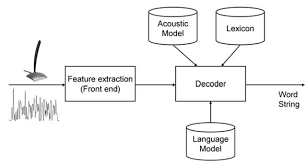
\includegraphics{asr}
\label{AutomaticSpeechRecognition}
\centering
\end{figure}

Picture \ref{AutomaticSpeechRecognition} shows an illustration how the automatic speech recognition works. ASR receives acoustic speech inputs and outputs a word string. An automatic speech recognition is composed of three components: acoustic model, language model, and lexicon. Acoustic model is a statistical model which represents a relationship between an acoustic input and its corresponding phonemes. Phoneme is a unit (or a group) of sound, for example: /k/, /l/, /sh/, etc. Lexicon is a dictionary which maps from words to their phonemes.  Language model computes the probability of a word string. Hence, the lexicon is used by the acoustic model and the language model together.  These three components work together to  search the most likely word sentence(from all possible sentences) which represents what people said in the audio. 


% talking about data: internet, partially closed caption, some has bad \textit{closed captions}
Despite of the rapid development of speech recognition, there are still many challenges in the field. One of the challenges is training a speech recognizer or adapting a speech recognizer to a new task which requires a massive amount of \textit{transcribed} training data. The \textit{transcribed} training data is audio data which has corresponding transcriptions what people said in the audio data. However, transcribing audio manually is labor intensive and also time consuming. There exist many unlimited supply of training data sources from internet, TV broadcasts, radio, as well as video streaming websites, like Youtube.  Nevertheless, many of them only possess few corresponding transcriptions or no transcription at all. To build a speech recognition, we can use a training dataset from TV broadcasts which usually have \textit{closed captions}. \textit{closed captions} are close, but not exactly the same as what people said. Furthermore, \textit{closed captions} are often badly aligned with the audio. These are some examples of good and bad \textit{closed captions},  as well as noisy utterance.
\begin{enumerate}
\item An example of good \textit{closed caption}. This segment/utterance has the same \textit{closed caption} as the detailed transcription.  
\begin{itemize}
\item Real transcription: \tab That is the very big question that leads to another big question. We're definitely thinking about putting an offer. That's great. 
\item \textit{Closed caption}:  \tab That is the very big question that leads to another big question. We're definitely thinking about putting an offer. That's great.
\end{itemize}


\item An example of bad \textit{closed caption}. The \textit{closed caption} is slightly different compared to the real transcription.
\begin{itemize}
\item Real transcription: \tab Russia started badly with the dropping at the hands of Spain. But, they got better and better. Spain looked unstoppable to start with but since then they have looked a little.
\item \textit{Closed caption}: \tab Russia started badly with at beating at the hands of Spain. Spain looked then they have looked a little
\end{itemize}


\item Noisy segment. Real transcription: Some segments in training audio may have background noise which makes it hard to be recognized by the ASR. Even, it is sometimes difficult to be recognized by humans. \\

[Clapping in the background] John Higgins developed very well. He is not five in front.[Still continues clapping in background]

\end{enumerate}

This internship explored how to build a high performance speech recognition system by utilizing less supervision because we did not have correct transcription audio data. The main idea is to use an automatic speech recognizer to automatically transcribe audio data which can be leveraged as a training dataset.  The steps of the main idea are as following: firstly, train on all data which are automatically \textit{transcribed} by other ASR systems, recognize these data with the ASR which we trained, and then compare the decoding transcriptions with the \textit{closed captions}. Finally, remove all segments which do not agree and train only the segments which agree.

The idea of using \textit{untranscribed} data(or \textit{unsupervised} training) has been proposed by Zavaliagkos and Colthurst in 1998\cite{Zavaliagkos1998UtilizingUT}, Kemp and Waibel in 1999 \cite{Kemp_unsupervisedtraining}. However, they only utilized small amount of data. Lamel et al were the first who proposed lightly supervised training data with a large amount of training data \cite{lightlySupervised}. In place of utilizing \textit{untranscribed} data, they trained  speech recognition systems by using audio data with \textit{closed captions}. The process is called lightly supervised approach.

%Therefore, selecting "good" data(audio data with very close captions) might be a solution to achieve a high performance ASR.

\textit{Lightly supervised} approach is one of the technique to select "good" data. An acoustic model from another task(or another corpus) is utilized to recognize audio data. The decoding results are compared with the \textit{closed captions} and removed if they disagree. These selected data are trained to generate a new acoustic model which is leveraged to recognize the same or different data. These decoding results are selected again for training a new acoustic model. This internship mainly focuses on the acoustic model component.

 The first goal of this internship is to study and evaluate the state-of-the-art techniques to select the "good" training data. The second goal is to propose new solutions to select data. The outcome of this internship will be useful as a training dataset to build a high performance automatic speech recognition.

%\section{About the project}

%Kaldi framework helps to train acoustic models with deep neural network in this internship. The  goals of the internship are as following:
%\begin{enumerate}
%\item Learn the state-of-the-art automatic speech recognition. I learn how to train and employ deep neural network for recognizing audio as well as build N-Gram language models. Moreover, I utilized a cluster computing server to train the acoustic models with massive amount of data.
%\item Select the subset of data which are close to the real transcription and evaluate how good our data selection is. The good data must have the \textit{closed captions} which are close to the real transcription.
%\item Propose new solutions which improve the current state-of-the-art.
%\end{enumerate}

This internship is expected to contribute in solving data selection problem. Internet has infinitely many audio data, for example: podcast, internet radio, tv broadcast, as well as video streaming. But, mostly they do not have transcriptions at all. In this internship, we conceived speech recognition systems by utilizing TV broadcasts and their corresponding \textit{closed captions}. 
%In the future, we hope that we use audio data without any transcription as the training dataset.

\section{Contributions}
We make several contributions as following:
\begin{enumerate}
\item We give some backgrounds related to speech recognition which helps the readers to understand how the speech recognition works in the nutshell. This background helps to grasp the idea of data selection.
\item We did some literature reviews and proposed some data selection methods.
\item  We implemented and evaluated some state-of-the-art data selection techniques. 
\item We implemented and evaluated new approaches in data selection and assessed these approaches against the current state-of-the-art approach. 
\end{enumerate}

\section{Outlines of the thesis}
This report is organized as following. In chapter 2, we elaborate some backgrounds in the automatic speech recognition. The chapter gives necessary backgrounds to the readers how speech recognition works; moreover, the  data selection method is further explained. Chapter 3 elaborates the data selection technique which was explored and experimented in this internship. Furthermore,  the new data selection methods are also proposed. Chapter 4 tells the setup of experiment and evaluation measurement. Then, chapter 5 shows the result of experiments. Lastly, the report is concluded by chapter 6 which conveys conclusion and some suggestions for future works. 

\chapter{Background}

\section{Automatic speech recognition}
\label{subsec:ASR}
The goal of the automatic speech recognition(ASR) is to search the most likely sentence($\hat{W}$) in a language $L$ given acoustic observation $O$ \cite{Jurafsky:2009:SLP:1214993}. ASR has been applied in many applications and domains, for example: automatic closed captioning for hearing-disabled persons \cite{Patel2010}, taking notes of conversations between doctors and patients \cite{Klann2008}, automatic closed captioning TV broadcasts \cite{Woodland2015}, and many more.

Observation $O$ can be seen as a sequence of sliced acoustic signal. Each successive index represents the consecutive slices of acoustic input.
\begin{equation}
O=o_{1},o_{2},o_{3},...,o_{t}
\end{equation} 
A sentence is composed of a sequence of words.
\begin{equation}
W = w_{1},w_{2},w_{3},...,w_{n}
\end{equation}


Thus, an automatic speech recognition can be formalized as following:
\begin{equation}
\label{asrEq}
\hat{W} = \textrm{argmax}_{W \in L} P(W|O)
\end{equation}

Applying the bayes rule to the equation \ref{asrEq} produces the equation bellow. Because observations $O$ do not change for every possible sentence, we can assume $P(O)$ as a constant and ignore it.
\begin{align}
\hat{W} & = \textrm{argmax}_{W \in L} \textrm{ } \frac{P(O|W) \times P(W)}{P(O)} \\
	& = \textrm{argmax}_{W \in L} \textrm{ } P(O|W) \times P(W)
\end{align}
where $\hat{W}$ is the most likely sentence, $P(W)$ is the prior probability of sentence $W$ computed by the language model, and $P(O|W)$ is the observation likelihood calculated by the acoustic model. This internship mainly focuses on the acoustic model. We will discuss the language and acoustic model more in the next subsection. 



\section{N-Gram Language model}


A language model is a statistical model which computes the probability of word sequence. One of the most common language model is N-gram language model, which we leverage in this internship. The foundation mathematics of N-Gram language model was proposed by Markov in 1913. Then, Shannon re-introduced N-gram to compute the likelihoods of English word sequences \cite{Shannon:2001:MTC:584091.584093}. N-gram language model has been applied in many applications, such as: speech recognition\cite{Woodland2015}, handwriting recognition \cite{Poznanski2016}, as well as spelling correction \cite{Kukich1992}.

The goal of language model is to compute the probability ($P(w|h)$) of a word $w$ given previous word history $h$ . The way to compute this probability is by using a large corpus and count the relative frequencies. For example: to count the word $w_{1}$ given history: $w_{2}, w_{3}, ..., w_{n}$, the probability is as following:
\begin{equation}
P(w_{1}|w_{2}w_{3}...w_{n})= \frac{C(w_{1}w_{2}w_{3}...w_{n})}{C(w_{2}w_{3}...w_{n})}
\end{equation}

Because we can create infinitely possible sentences, it is more efficient to compute probability by applying the chain rule of probability. 
\begin{align*}
P(w_{1}^{n}) & =P(w_{1})P(w_{2}|w_{1})P(w_{3}|w_{1}^{2})...P(w_{n}|w_{1}^{n-1}) \\
& = \Pi_{k=1}^{n} P(w_{k}|w_{1}^{k-1})
\end{align*}

However, the probability of a word given preceding words is infeasible to be computed. Instead of computing the entire preceding history, N-gram only approximates the probability with last few words. For example: the bigram LM approximates the probability of a word given history by the probability of a word given the last word only $P(w_{n}|w_{n-1})$.  This approximation(or assumption) is called Markov assumption.

A major problem exists in N-Gram language model. Information inside a corpus might be limited. Some word sequences probably do not exist in the corpus, but they are perfectly acceptable word sequences. If we calculate the N-Gram likelihood for these sequences, we will get zero value. The solutions to the problem are backoff and smoothing. Backoff allows the N-gram LM to use the value of lower N-Gram LM if we have zero probability in the higher N-Gram.  Smoothing is a technique to avoid  zero probability for every word sequence. If a word sequence does not exist in the corpus, the LM still produces a non-zero value even though it is small. We used Kneser-Ney smoothing \cite{KneserNey1993} which has been implemented in SRILM framework.

To evaluate the performance of a language model(LM), perplexity can be applied to the LM. The intuition behind LM is given two N-gram LM, the better model is the one which predicts test set better than the other. Lower perplexity means that the model is better. Given a language model and a test corpus, perplexity is calculated as following \cite{Bahl:1983:MLA:2053027.2053281} \cite{Klakow:2002:TCW:638078.638080}:
\begin{equation}
PP = exp(-\frac{1}{N} \sum^{N}_{i=1} \log P(w_{i}|h_{i}))
\end{equation}
where $N$ is the number of words in test corpus, $w_{i}$ is the i-th word, and $h_{i}$ is the history of word $w_{i}$.


\section{Acoustic model}
The acoustic model(AM) is commonly based on hidden markov model(HMM). Thus, before talking about the acoustic model deeply, it is better to elaborate HMM first. 


\subsubsection{Markov chain}
A weighted state finite automaton is a finite state automaton where the arc between nodes has probability how likely the path is taken. Markov chain is one kind of weighted state finite automata which the input sequence determines which state the automaton will go.

Markov chain can be defined formally as following:
\begin{itemize}
\item $Q=q_{1}q_{2}...q_{N}$ a set of states
\item  $A=
\begin{bmatrix}
a_{01}a_{02}a_{03}...a_{0n} \\
a_{11}a_{12}a_{13}...a_{1n} \\
... \\
a_{01}a_{02}a_{03}...a_{0n} \\
\end{bmatrix}
$ is a transition probability matrix where $a_{ij}$ represents the probability of moving from state $i$ to state $j$. In addition to that, the sum of outgoing probability of every state must be summed into 1. $\sum_{j=1}^{n}  a_{ij}=1$. 
\item $q_{0}$ and $q_{F}$ represent initial and final states.
\end{itemize}

\subsubsection{Hidden markov model(HMM)}
\label{HMM}
Markov chain is only usable if the event is directly observable in the world. However, we are interested in some events which are not observable or hidden for some problem. For example: acoustic event is observable, but word event is not observable in speech recognition problem. Hidden markov model fixes this problem. 

Hidden markov model is formalized as 
\begin{itemize}
\item $Q=q_{1}q_{2}...q_{n}$ is a set of states
\item  $A=
\begin{bmatrix}
a_{01}a_{02}a_{03}...a_{0n} \\
a_{11}a_{12}a_{13}...a_{1n} \\
... \\
a_{01}a_{02}a_{03}...a_{0n} \\
\end{bmatrix}$ is a transition probability matrix where $a_{ij}$ represents the probability of moving from state $i$ to state $j$ such that $\sum_{j=1}^{n}  a_{ij}=1$ for every $i$.
\item $O=o_{1}o_{2}...o_{T}$ is a sequence of $T$ observations.
\item $B=b_{i}(o_{t})$ is observation likelihoods(or emission probability) where state $i$ emits probability given observation $o_{t}$. 
\item $q_{0},q_{F}$ are initial and final states.

Hidden markov model employs two assumptions:
\begin{enumerate}
\item Markov assumption. The state is only dependent to the previous state.
\begin{equation}
P(q_{i}|q_{1}q_{2}...q_{i-1}) = P(q_{i}|q_{i-1})
\end{equation}
\item Output independence assumption. Output observation $o_{i}$ is only dependent with the state $q_{i}$ which produces $o_{t}$ and independent with other states and other observations.
\begin{equation}
P(o_{i}|o_{1}o_{2}...o_{i}..o_{T}q_{1}q_{2}...q_{i}..q_{N}) = P(o_{i}|q_{i})
\end{equation}

\end{enumerate}

\end{itemize}  

\subsubsection{Applying HMM to acoustic model}
In section \ref{HMM}, HMM is explained. Now, it is time to apply HMM on acoustic model. 
\begin{enumerate}
\item States \\
A state in acoustic model can represent a word, a phone, or a sub phone depending on the problem we are trying to solve. For the digit recognition problem, a state represents a sound of one number. A sequence of phone can be represented as a word string. Hence, for more complicated task, like recognizing TV broadcast, it is better to make a state representing a phone or even a sub phone. A sound of a phone is usually influenced by the preceding and successive phone. Therefore, we use three HMM states(for each phone) which capture beginning, middle, and  end of the phone. The sub phone state is commonly called as a senone.

\begin{figure}[H]
\caption{A triphone HMM model consisting of three emitting states(beginning(S0), middle(S1), and end(S2) of a phone), a transition matrix $A$, and emission probability(observation likelihood) $B$ \cite{SiliconAM}}

\includegraphics[scale=0.6]{tiphone}
\centering
\end{figure}

\item Transition matrix \\
The transition matrix in speech recognition is the probability of moving from the current sub phone state to the successive sub phone state. Unlike HMM, Speech recognition HMM does not allow arbitrary transition because of the sequential nature of language and speech. A state can go to itself or to the next states, but it can not go back to the preceding state. This kind of left-to-right constrained HMM is called Bakis network.

\item Observation \\
The observation is a sequence of acoustic feature vector. The acoustic input is divided into small chunks and converted into a feature vector.
%Acoustic feature vector is a 39-dimension which is generated based on Mel-frequency cepstral coefficient(MFCC). Each observation is a slice of 10 milliseconds audio. For one second audio, there will be 100 acoustic feature vectors where each vector has 39 features.

\item Observation likelihood \\
Observation likelihood is the probability of a feature vector which is generated by a sub phone state. 

\end{enumerate}


\section{Deep learning for acoustic model}
For our acoustic model, we used deep neural network(DNN) HMM. Beside DNN HMM, there exists gaussian mixture model(GMM) HMM. However, DNN HMM has been proven to outperform GMM DNN in practice \cite{Peddinti2015ATD}. Hence, we only discuss DNN in this report.

\subsubsection{Feedforward neural network}
Feedforward neural network(or sometimes called multilayer perceptron(MLP)) is one kind of neural network. MLP approximates function $f'(\mathbf{x})=\mathbf{y}$. MLP can be represented as $f(\mathbf{x};\mathbf{\theta})=\mathbf{y}$ and learn parameters $\mathbf{\theta}$ which maximizes function approximations. 

Perceptron is a kind of artificial neuron developed in 1960 by Frank Rosenblatt \cite{Rosenblatt1960}. A perceptron receives several inputs($x_{1}, x_{2}, ..., x_{n}$), does weighted sum $\sum_{i} x_{i}w_{i}$, and is thresholded by bias $b$ to make a decision: zero or one.
 
\begin{equation}
output = 
\begin{cases}
0 , \textrm{if } \sum_{i} x_{i}w_{i} + b \leq 0 \\
1, \textrm{if } \sum_{i} x_{i}w_{i} + b > 0
\end{cases}
\end{equation}

\begin{figure}
\label{tdnnArchitecture}
\caption{A perceptron}
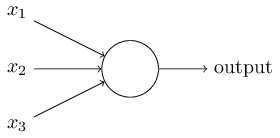
\includegraphics[scale=0.6]{perceptron}
\centering
\end{figure}

A perceptron is too simple to capture non linear pattern. Therefore, the perceptron is modified by applying an activation function into weighted sum. There are several common activation functions, such as: 
\begin{enumerate}
\item Sigmoid
\begin{equation}
a(x) = \frac{1}{1 + e ^{-x}}
\end{equation} 

\item Rectified linear unit(relu)
\begin{equation}
a(x) = max(0,x)
\end{equation} 


\item Softmax
\begin{equation}
a(x) = \frac{e^{x}}{\sum_{i} e^{x_{i}}}
\end{equation} 

\end{enumerate}

In addition to activation function, we need to make neuron to capture more complex features by stacking many neurons together. This network is called a feed forward multi layer perceptron. This neural network does not have connections between units which form a cycle. It is also called feedforward because the input values are propagated forward to output. The neural network receives inputs, does weighted sum, and applies activation function. The output of the units in one layer is propagated to the units in the next layer until reaching output layer. 

\begin{figure}[H]
\caption{Multi layer perceptron}
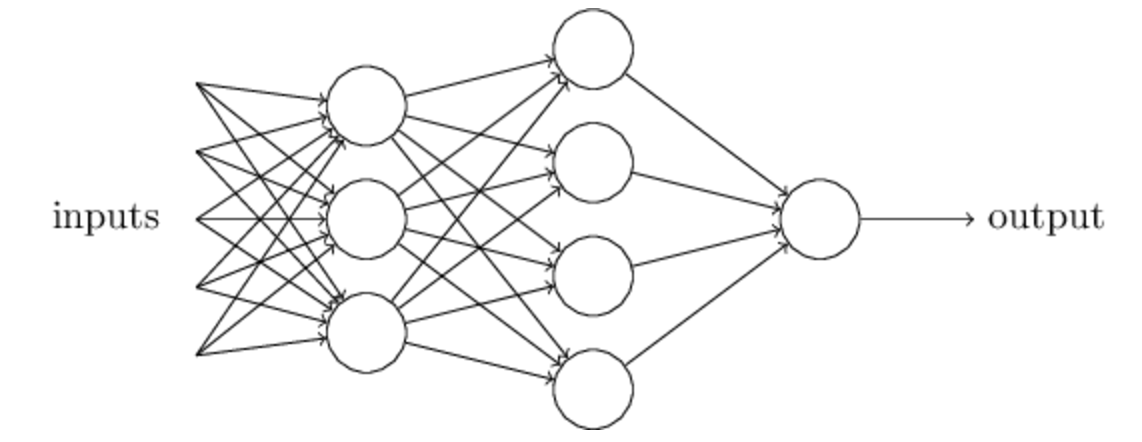
\includegraphics[scale=0.6]{mlp}
\centering
\end{figure}

\subsubsection{Time delay neural network(TDNN)}
To model a temporal sequence neural network, like the speech recognition problem, the model must have the following properties: it must have multiple layers to learn complex non linear decision surface, represents relationships between events in time, invariant under translation in time, and does not require precise temporal alignment. From all of these properties, time delay neural network(TDNN) qualifies to model a temporal sequence neural network.

There exist two ways to capture long temporal contexts:
\begin{enumerate}
\item Feature representation which present the information of long temporal contexts. The examples of the feature representation are TRAPs\cite{Hermansky99temporalpatterns}, multiscale spectro-temporal modulations representation\cite{Mesgarani04speechdiscrimination}, deep scattering spectrum representation\cite{Anden2014}, and modulation frequency feature representations\cite{Thomas2009}. These feature representations can use the standard feed forward deep neural network to model the temporal sequence neural network.

\item Acoustic model which can learn long temporal contexts and is trained on short-term feature representations. Recurrent neural network(RNN) \cite{1402.1128} and time delay neural network \cite{Waibel:1990:PRU:108235.108263} are two state-of-the-art acoustic models which are suitable to model this acoustic model. 
\end{enumerate}

Peddinti et al showed that TDNN performs better than RNN in term of parallelization during training\cite{Peddinti2015ATD}. Due to recurrent connections in RNN, RNN is not able to fully utilize parallelization in GPU(general processing unit) the same extent as TDNN. In addition, TDNN has been proven to have lower word error rate compared to RNN\cite{Peddinti2015ATD}. Thus, we will focus more on TDNN and trained acoustic models with TDNN in this internship.

Time delay neural network(TDNN) was first proposed by Waibel et al in 1990\cite{Waibel:1990:PRU:108235.108263}.TDNN is suitable to model long term temporal relationship within the range of $N$ delays in short term speech features; for example: MFCC feature representations. %todo explain more TDNN here

%The acoustic feature is called short term feature because it is an MFCC feature vector generated from a slice of 10 milliseconds acoustic input. 

\begin{figure}

\caption{An example of a TDNN architecture. \cite{Peddinti2015ATD}}
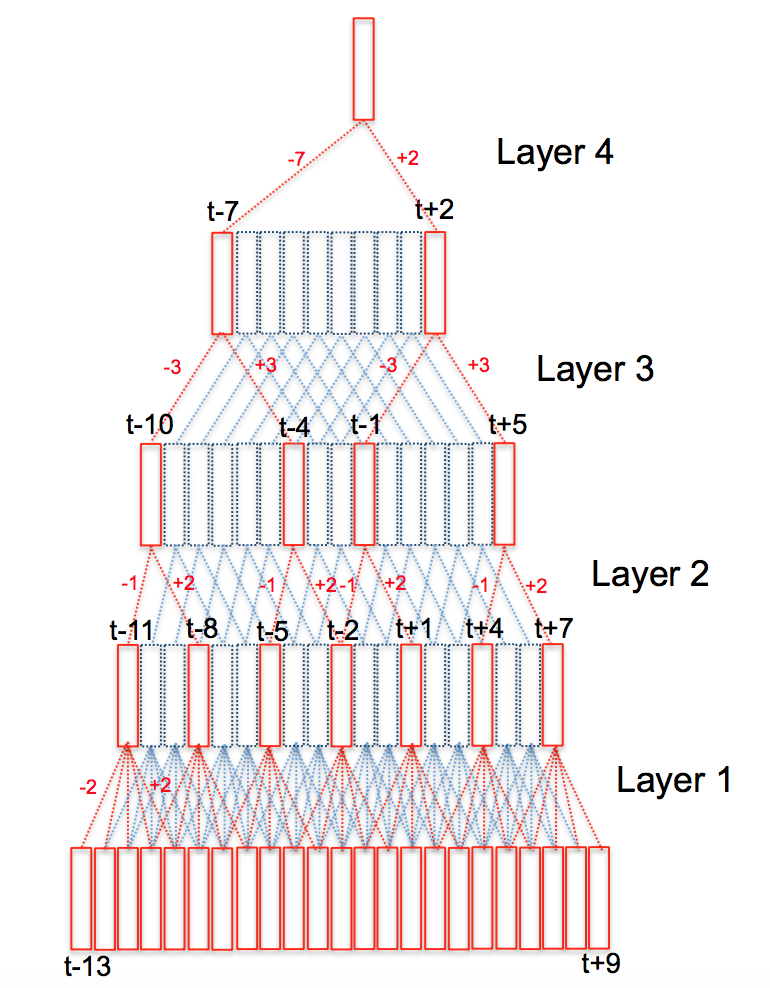
\includegraphics[scale=0.6]{tdnnArchitecture}
\label{tdnnArchitecture}
\centering
\end{figure}


%To learn sequential inputs, TDNN must learn sequence of cues. Hence, Waibel et al introduced a time delay $D_{1}$ to $D_{N}$ to learn long term temporal dependencies. The input feature vector is 40 dimensional MFCC feature vector. Figure \ref{tdnnArchitecture} shows the TDNN architecture. The input layer receives 4 delays($N=4$), i.e. $\{t-2, t-1, t, t+1, t+2\}$. Therefore, each unit has 200 weights($5 \times 40$) from input layer. The next layer(hidden layer 1) receives delay from $t-1$ through $t+2$. The higher layer will receive wider temporal contexts compared to the lower layers. For example, the final layer receives inputs which are time delay  from $t-7$ through $t+2$ context. 

TDNN is basically a feedforward neural network. Learning procedure which we used is backpropagation. There are two passes procedure in the backpropagation. The first pass is forward pass where the neural network receives input, does weighted sum, and applies activation function. The output values from the first layer is forward propagated until reaching the output layer. Then, square error is calculated between the expected value and the output of neural network. The second pass is backward pass where the derived square error value is propagated backward to update weights. 

Typical TDNN computes all hidden activation in each layer. Figure \ref{tdnnArchitecture} demonstrates an architecture of TDNN. TDNN receives acoustic inputs with some delays to the left and right contexts(before and after time $t$). Usually, the input context is asymmetric, i.e: more time context to the left than right. The main reasons are to reduce the latency of online decoding and improve word error rate. Each layer splice together contiguous temporal windows within a time range; for example: the third layer splices the frames within range $[t-3, t+3]$ in the figure  \ref{tdnnArchitecture}. Furthermore, TDNN applies wider splice when going to higher layers in the networks as shown in the figure \ref{tdnnArchitecture}. The reason is we force the higher layer to learn wider temporal contexts.

Training a TDNN is still time consuming. The standard TDNN computes all hidden activation in each layer. Consequently, the training time of TDNN is approximately ten times compared to the standard DNN.  Peddinti et al found that there exist large overlaps between input contexts at neighboring time steps; thus, they proposed subsampling \cite{Peddinti2015ATD}. The technique generally only splice no more than two temporal contexts with gap instead of contiguous temporal windows. Figure \ref{tdnnArchitecture} illustrates the procedure of subsampling. In the standard TDNN, all hidden units(red and blue) are calculated. In contrast with subsampling technique, only red hidden units are computed. In consequence, the training time of subsampled TDNN is approximately five times faster than the standard TDNN \cite{Peddinti2015ATD}. Moreover, subsampling is able to reduce the model size. Splicing contiguous temporal contexts will require a massive number of parameters. However, subsampling only splices less temporal contexts than the typical TDNN.

\subsubsection{Hybrid acoustic model}
\label{HybridAcousticModel}
To train a TDNN or other kinds of DNN acoustic model, one needs to label each acoustic input vector. However, our initial data only have utterance level of start and end time. Even, each word does not have start and end time. Each acoustic input must be labeled with its corresponding senone in order to train a DNN-HMM acoustic model. 

GMM acoustic model can bootstrap the labeling process\cite{1406.7806}. We can train a GMM-HMM acoustic model with flat start, i.e: without previous phoneme-to-audio alignment.  Therefore, the step before training a DNN acoustic model is by training a GMM-HMM acoustic model. Then, force align the training set with the acoustic inputs to generate a sequence of senone which corresponds with the transcription in the segments. The aligned data(the acoustic input with its corresponding senone) is utilized to train a DNN acoustic model.

Training a DNN-HMM is a little bit different than the HMM as explained in \ref{subsec:ASR}. An acoustic model usually models the probability $P(o|y)$ of observation(acoustic input) $o$ given its corresponding senone $y$. Nonetheless, DNN models the probability of a senone given the observation $P(y|o)$. By applying the bayes rule, $P(o|y)$ can be obtained as the following:
\begin{equation}
P(o|y)  = \frac{P(y|o) \times P(o)}{P(y)}
\end{equation}
$P(y)$ can be obtained from distribution of a senone in the training set. By using lexicon, each word in the training set can be mapped into the corresponding senone. However, $P(o)$ is infeasible to be obtained. Luckily, the observation $o$ are fixed and can be seen as a constant. Hence, we can provide HMM with the unnormalized probability..
\begin{equation}
\frac{P(y|o) }{P(y)}
\end{equation}

Applying the hybrid approach has been introduced over 20 years ago \cite{Bourlard:1993:CSR:562393,Renals1994}. Nevertheless, it did not outperform GMM until recently. DNN reduces substantial amount of word error rate compare to GMM \cite{Dahl2011,38130}. DNN excels in improving accuracy due to more representational capacity compared to GMM \cite{1406.7806}. There are several factors why DNN outperforms GMM just recently.
\begin{itemize}
\item The amount of training dataset has increased. DNN usually works well when there exists a massive volume of training data.
\item Training DNN can be done on GPU which accelerates the execution time. 
\item We have more powerful neural network architecture recently with more number of parameters, more hidden layers(deeper network), and better initialization procedure. 
\end{itemize}

% It subsamples $t-1$ and $t+2$ time(without including $t$ and  $t+1$ time samples) in the second layer, subsamples $t-3$ and $t+3$ in the third layer, and subsamples $t-7$ and $t+2$ in the final layer. 

% advantage of TDNN is it can reduce computational time and model size.

%\section{Lexicon}


\chapter{Methodology}

\section{Data selection: Lightly supervised approach}
Despite of the high development in automatic speech recognition, there exist many challenges. One of the main challenge of speech recognition is to reduce development cost when adapting the speech recognition to other task or creating a new speech recognition for a new language. The biggest development cost is to transcribe the audio data with their exact corresponding transcriptions. To generate a "good" speech recognition, one needs a massive number of training audio and their exact transcriptions. However, transcribing audio is labor intensive and time consuming too. There are unlimited supply of audio data in the internet, television, radio, and other sources. Nonetheless, they usually have a few or even no accurate transcription at all.  Some television broadcasts have corresponding closed captions.  Closed caption means that the transcription is close, but not exactly the same as what the audio says. Even, the closed captions are often badly time-aligned with the audio.

By utilizing these audio data with the corresponding closed captions, we hope to produce a high performance speech recognizer with less supervision. The main idea is to use the automatic speech recognizer to transcribe audio data which will automatically generate transcriptions, which later be used as training data \cite{lightlySupervised}. The steps are as following. Firstly, we train a bootstrap acoustic model trained on a small manually annotated data. Then, recognize the data with closed captions by using the bootstrap model. We compare the decoding result from the bootstrap model with the closed captions and remove the words which do not agree. Finally, we can train a new acoustic model from the filtering.

The idea of using untranscribed audio data has been explored before(Zavaliagkos and Colthurst in 1998 \cite{Zavaliagkos1998UtilizingUT} and Kemp \& Waibel \cite{Kemp_unsupervisedtraining}), which is called as unsupervised acoustic model training. They utilized small amount of audio data without transcription to train acoustic models. The drawback of their experiments is not using massive volume of training data which is essential to train an acoustic model.

Lightly supervised approach was proposed in 2002 by Lamel et al \cite{lightlySupervised}. 
In general, the lightly supervised approach operates as following:
\begin{enumerate}
\item Train an acoustic model on a small amount of manually annotated data. 
\item Recognize(or automatically transcribe) a massive amount of data.
\item Align the automatic transcriptions with the closed captions. Some transcriptions and closed captions might disagree. We can remove or correct these segments.
\item Retrain a new acoustic model using the data which we selected in the previous step. 
\item Reiterate from step 2.
\end{enumerate}
These steps can be iterated several times as long as the error rate is decreasing. This method uses the idea of training acoustic model in less supervised manner because the training dataset(closed captions) is not the real detailed transcription. 

Using closed caption as training data reduces effort in manual transcription.Detailed transcription process usually takes 20-40 times manual effort compare to live closed captioning. Closed caption is usually produced in real time and less costly compare to the detailed transcription. In addition, the manual transcription is possible to have error \cite{Barras2001}. Additionally, some TV broadcasts, such as: CNN headline news, ABC world news tonight, BBC, already have closed captions which can be used as a training dataset. Nevertheless, some problems exist when using the data with closed captions as training dataset. However, training using  the closed captions faces several disadvantages compared to the real transcriptions: indication of non speech event, such as: coughing, speaker turn, acoustic conditions: background noise and music. Furthermore, some sentences might be paraphrased, deleted, and changed in word order. 

In addition to the closed captions, we can use additional data to build a language model. Other kinds of text are available in internet, such as: news, blog, and closed captions from TV broadcast. However, these data might be less related with the audio data. Some additional sources may be not contemporaneous with the data. Thus, it provides less supervision. We can interpolate these data with the closed captions to build a more general language model.

Despite the fact that closed captions are not accurate, it has been proven that closed captions provides enough supervision in building automatic speech recognition systems \cite{lightlySupervised}. Lamel found that an increase in training data improves accuracy even tough it will increase the model size. Additionally, filter closed captions for the next iteration training set in the lightly supervised technique improves the accuracy slightly. The language model built from closed captions also effectively provides enough supervision in building the ASR. Therefore, lightly supervised technique is our main inspiration to do data selection in this internship.

\section{State-of-the-art data selection}
Some researches have been conducted to investigate the lightly supervised approach to select data in the speech recognition problem\cite{lightlySupervised,Lecouteux06imperfecttranscript,Chan,Mathias,Stolcke00anefficient}. The state-of-the-art data selection was proposed by  Lanchantin et al from Cambridge university\cite{Lanchantin2016}. Before talking about the state-of-the-art, it is better to discuss some previous related works first.

Lamel et al proposed the lightly supervised approach which harnessed the closed caption as supervision to build a robust speech recognizer\cite{lightlySupervised}. In their experiment, they used a bootstrap acoustic model and biased language model to recognize the audio where the decoding result is compared with the closed caption. Then, the words which do not agree will be removed from training dataset. The new training dataset is utilized to train a  new acoustic model. This filtering(removing not-agree words) is called closed caption filtering.

Chan and Woodland explored another way in filtering bad closed captions\cite{Chan}. They leveraged the confidence measure metric to remove the bad segments. When decoding acoustic inputs, an ASR produces word hypothesis and their corresponding confidence measure. The confidence measure value from each word in  each segment is averaged to produce one confidence value per segment. Finally, they determined a threshold confident value to filter out all potentiallly bad segments, where the confident value is lower than the threshold. Moreover, they also introduced to interpolate two different LMs created from two closed caption datasets and merge them into one single LM. This single LM is used as light supervision when decoding acoustic input together with the acoustic model and the lexicon.

Matias et al applied lightly supervised approach on medical conversation data \cite{Mathias}. There are unlimited supplies of medical speech; however, only informal medical reports are available. The medical reports are not the same as what the physicians said in the audio records. This problem matches perfectly with the lightly supervised approach. They explored frame level filtering in place of word level or segment level filtering. Basically, they forced align and compared the decoding results with the closed captions and mark words which are insertion, deletion, and substitution. All corresponding frames which are associated with those marked words are removed or filtered out from training set to produce a new cleaner training set.

The state-of-the-art data selection was proposed by  Lanchantin et al from Cambridge university\cite{Lanchantin2016}. They used the lightly supervised approach applied on the multi genre broadcast(MGB) challenge. MGB challenge is a challenge to automatically transcribe TV broadcasts. The challenge only provided TV broadcast audio data and their corresponding closed captions. General TV broadcast data are usually recorded in highly diverse environment speech with background music, non speech event, and sound effect. In addition, some closed captions may be different compared to the real transcription due to deletion, insertion, substitution, and paraphrasing. These factors make the challenge interesting as well as complicated. 

Lanchantin et al proposed to tackle the problem inspired from the lightly supervised approach. The lightly supervised approach works as following \cite{Lanchantin2015}.
\begin{enumerate}
\item Trained an acoustic model by selecting a subset of 200 hours training set from the total 1600 hours training set. We called this as AM-v1 which is based on deep neural network.
\item AM-v1 recognized the entire training dataset(1600 hours) which resulted in the decoding result. Compare and force aligned the decoding result with the closed captions. By comparing each segment, they calculated phone matched error rate(PMER) and word  matched error rate(WMER) as well as average word duration.
\item By utilizing average word duration and phone matched error rate, they selected 700 hour of data(700hr-v1). The way to select the data is 
\begin{enumerate}
\item Reject segments which are not in the range of $0.165 \leq AWD \leq 0.66$
\item Sort segments based on PMER and select the top segments until reaching 700 hours set. The threshold for this iteration is $40\%$. This new selected training data is called 700-v1.
\end{enumerate}
\item Retrain a new acoustic model using the 700-v1. Repeat step 2-4 to create 700-v2, 700-v3 until the data selection algorithm converges. 
\end{enumerate}

In every iteration, the language model which they utilized are the same. MGB provides closed captions for each audio and additional text consisting 10 million and 640 million words respectively. From these texts, two language models were built and interpolated into one language model. Furthermore, the merged language model was pruned by $10^{-9}$ to expedite the decoding process.

A question remains to be asked: when to stop the iteration(the algorithm converges)? The MGB challenge provides a development set which comprises of audio data and their manually transcribed transcriptions. These transcriptions are exactly what people said in the audio with correct time stamp. By recognizing the development set with the ASR system which they built in each iteration, they calculated word error rate(WER). If the WER decreases in the next iteration, continue the iteration. Otherwise, stop the iteration.






\section{Data}
Before talking about the methodology, it is better to talk about the dataset. We have the following dataset:
\begin{enumerate}
\item Training set has audio data with their corresponding closed captions.
\item Test set has audio data and their corresponding manual transcriptions. These manual transcriptions are the same as what people said in the audio.
\item Additional text corpus which is utilized for building language model. This additional corpus is different than the closed captions in training set. 
\end{enumerate}




\section{Language model}



\section{Acoustic model}

\section{Data selection}

%\textbf{Insert time and perpelexity here.}

\section{Baseline model}

\subsection{Acoustic model AM.200 and Language Model Version 1 (LM.200.1e-9)}
\label{amv0s1}


Calculating PMER and WMER for each segment by utilizing AM.200 and LM.200.1e-9:
\begin{enumerate}
\item GMM(GMM.200): GMM is trained by using the 200 hours data
\item TDNN(TDNN.200): the result of GMM training(GMM.200) is utilized to build a TDNN(time delay neural network). 
\item TDNN graph creation \\
The language model used is the LM.200.1e-9 and  the acoustic model is  TDNN.200; furthermore, the dictionary used(Lexicon.200) is the modification of the library provided by MGB(Lexicon.MGB). Words in Lexicon.MGB which do not exist in word.200 are removed from Lexicon.200.
%\item TDNN development set recognition \\
%The development set is files from dev.short, which contains 8 hours of audio. The development set is recognized by leveraging the graph created in the previous step.
\item TDNN 200 hours of training data recognition \\
We need to recognize 200 hours data to calculate PMER, WMER, and AWD. This data will be used for data selection of the next iteration.
\item Sclite score PMER and WMER \\
Use the lattice and graph(produced at step 5 and 3 respectively) to calculate overall PMER and WMER. However, the decoding program does not provide PMER, WMER, and AWD for each segment. Fortunately, the program generates prf file which contains number of correction, insertion, deletion, and substitution for each segment. Two prf files exist after decoding:(ctm\_words.filt.filt.prf contains word match error rate and ctm\_phones.filt.filt.prf contains phone match error rate). From there, we are able to calculate  PMER, WMER, and AWD of each segments.  For the development set, we only need to know the overall PER and WER. In contrast, training set recognition needs PMER, WMER, and AWD for each segment. 

\end{enumerate}


version AM0
% table
\begin{center}
\begin{tabular}{ | c | c | c | c |  c |  }
\hline
\textbf{No.} & \textbf{Description} & \textbf{Result} & \textbf{execution time} & \textbf{extra info} \\ \hline \hline
1 & GMM.100  &  & 3h 30m & 20 hosts \\  \hline
%/talc2/multispeech/calcul/users/jkarsten/mgb/recipe/tools/baseline/baseline1_backup/gmm
%1.1 & GMM decoding & 57.2\% WER  & 3h 36m 47s & 20 hosts, 4 cores \\  \hline \hline
%2 & AM.200 training. &  & 38h 30m 31s & 3 nodes \\  

2 & TDNN.100 training: & & 17h 7m & 3 GPU hosts \\ 
 & LM.200.1e-9,  GMM.100, Lexicon.200 &  & & \\ \hline
 %/talc2/multispeech/calcul/users/jkarsten/mgb/recipe/tools/baseline/baseline1_backup/tdnn
 
3 & Create a graph from TDNN.200,  &  & 6m & 1 host \\  
 & LM.200.1e-9, Lexicon.200  & & & \\ \hline
%/talc2/multispeech/calcul/users/jkarsten/mgb/recipe/tools/modifASR/tdnn_s1/graph_creation_from_arpaLM

4 & Create a graph from TDNN.200,  &   & 4h 49m & 1 host \\  
 & LM.7weeks+subtitles.1e-9, Lexicon.200  & & & \\ \hline

%4 & AM.200 recognized dev.short &  & 2h 58m 58s   & 20 hosts  \\  \hline
5 & TDNN.100 recognized train.200 &  & 16h 6m & 20 hosts \\  \hline 
 %/talc2/multispeech/calcul/users/jkarsten/mgb/recipe/tools/modifASR/tdnn_s1/recognition_with_scoring/decode_res_train_200_fst+merall_mgb2015.wordList.4gm.kn.arpa.gz.1e-9.arpa_4thr

6 & TDNN.100 \& LM.7weeks+subtitles.1e-9 & WER 43.9\%   & 45m & 20 hosts \\  
&  recognized dev.short & PER 35.8\% & & \\ \hline
%5 & Calculate Overall PMER & 24.8 \% PMER   & 5h 5m 51s & 1 host \\  \
 %& and WMER of train.200  & 32.4 \% WMER & & \\ \hline
%5.1 &  Calculate PMER and WMER & & 20m 22s & 1 host \\  
 %&  per segment of step 6 & & &  \\  \hline
%/talc2/multispeech/calcul/users/jkarsten/mgb/recipe/tools/modifASR/tdnn_s1/sclite_score_pmer_and_wmer
% /talc2/multispeech/calcul/users/jkarsten/mgb/recipe/tools/modifASR/tdnn_s1/calculate_pmer_wmer_per_segments

%6 & Calculate PER  &  32.5 \% PER  & 1h 10m 57s   & 1 host \\  \
% & PMER, WMER calculation  &   48.7\% WER   & & \\ \hline
\end{tabular}
\end{center}


%%%%%%%%%%%%%%%%%%%%%%%%%%%%%%%%%%%%%%%%
% table
version AM1
\begin{center}
\begin{tabular}{ | c | c | c | c |  c |  }
\hline
\textbf{No.} & \textbf{Description} & \textbf{Result} & \textbf{execution time} & \textbf{extra info} \\ \hline \hline
1 & GMM.100  &  & 4h 7m & 20 hosts \\  \hline

2 & TDNN.100 training: & & 20h 1m & 3 GPU hosts \\ 
 & LM.200.1e-9,  GMM.100, Lexicon.200 &  & & \\ \hline
 
3 & Create a graph from TDNN.200,  &  & 5m & 1 host \\  
 & LM.200.1e-9, Lexicon.200  & & & \\ \hline
 
4 & Create a graph from TDNN.200,  &   & 3h 7m & 1 host \\  
 & LM.7weeks+subtitles.1e-9, Lexicon.200  & & & \\ \hline

5 & TDNN.100 recognized train.200 &  & 14h 18m & 20 hosts \\  \hline 

6 & TDNN.100 \& LM.7weeks+subtitles.1e-9 & WER 41.2\%   & 46m & 20 hosts \\  
&  recognized dev.short & PER 33.8\% & & \\ \hline
\end{tabular}
\end{center}

%%%%%%%%%%%%%%%%%%%%%%%%%%%%%%%%%%%%%%%%
version AM2
\begin{center}
\begin{tabular}{ | c | c | c | c |  c |  }
\hline
\textbf{No.} & \textbf{Description} & \textbf{Result} & \textbf{execution time} & \textbf{extra info} \\ \hline \hline
1 & GMM.100  &  & 3h 3m & 20 hosts \\  \hline

2 & TDNN.100 training: & & 23h 58m & 3 GPU hosts \\ 
 & LM.200.1e-9,  GMM.100, Lexicon.200 &  & & \\ \hline
 
3 & Create a graph from TDNN.200,  &  & 5m & 1 host \\  
 & LM.200.1e-9, Lexicon.200  & & & \\ \hline
 
4 & Create a graph from TDNN.200,  &   & 3h 13m & 1 host \\  
 & LM.7weeks+subtitles.1e-9, Lexicon.200  & & & \\ \hline

5 & TDNN.100 recognized train.200 &  & 15h 51m & 20 hosts \\  \hline 

6 & TDNN.100 \& LM.7weeks+subtitles.1e-9 & WER 40.5\%   & 36m & 20 hosts \\  
&  recognized dev.short & PER 33.3\% & & \\ \hline
\end{tabular}
\end{center}


%%%%%%%%%%%%%%%%%%%%%%%%%%%%%%%%%%%%%%%%
version AM2
\begin{center}
\begin{tabular}{ | c | c | c | c |  c |  }
\hline
\textbf{No.} & \textbf{Description} & \textbf{Result} & \textbf{execution time} & \textbf{extra info} \\ \hline \hline
1 & GMM.100  &  & 3h 3m & 20 hosts \\  \hline

2 & TDNN.100 training: & & 25h 27m & 3 GPU hosts \\ 
 & LM.200.1e-9,  GMM.100, Lexicon.200 &  & & \\ \hline
 
3 & Create a graph from TDNN.200,  &  & 7m & 1 host \\  
 & LM.200.1e-9, Lexicon.200  & & & \\ \hline
 
4 & Create a graph from TDNN.200,  &   & 4h 49m & 1 host \\  
 & LM.7weeks+subtitles.1e-9, Lexicon.200  & & & \\ \hline

5 & Create a graph from TDNN.200,  &   & 2h 1m each genre & 1 host \\  
 & LM.genres.1e-9, Lexicon.200  & & & \\ \hline

6 & TDNN.100 recognized train.200 &  & 15h 52m & 20 hosts \\  \hline 

7 & TDNN.100 \& LM.7weeks+subtitles.1e-9 & WER 40.5\%   & 38m & 20 hosts \\  
&  recognized dev.short & PER 33.3\% & & \\ \hline
\end{tabular}
\end{center}



%\subsection{Acoustic model AM.200 and Language Model LM.7weeks+subtitles.limited.1e-9}
% table
%\begin{center}
%\begin{tabular}{ | c | c | c | c |  c |  }
%\hline
%\textbf{No.} & \textbf{Description} & \textbf{Result} & \textbf{execution time} & \textbf{extra info} \\ \hline \hline
%3 & Create a graph from TDNN.200,  &  & 3h 12m 25s & 1 host \\   
% & LM.7weeks+subtitles.limited.1e-9,   & & & \\ 
% & Lexicon.7weeks+subtitles & & & \\ \hline
 %/talc2/multispeech/calcul/users/jkarsten/mgb/recipe/tools/modifASR/tdnn_s2/graph_creation_from_arpaLM


%4 & TDNN.200 &  & 1h 10m 59s & 20 hosts \\  
% & recognized dev.short & & & \\ \hline
% /talc2/multispeech/calcul/users/jkarsten/mgb/recipe/tools/modifASR/tdnn_s2/recognition_human/recognition_with_scoring_human


 %5 & TDNN.200 recognized &  & 10h 9m 35s & 20 hosts \\  
 %& train.200 & & & \\ \hline  
 %/talc2/multispeech/calcul/users/jkarsten/mgb/recipe/tools/modifASR/tdnn_s2/recognition_with_scoring
 
% 6 & TDNN AM.200 dev short & 31.8\% PER  & 4h 58m 26s & 1 hosts \\  
% & PMER, WMER calculation & 49.5\% WER & & \\ \hline
% 6.1 & TDNN AM-V0 train 200 & 26.4\% PMER & 4h 58m 26s & 1 hosts \\  
% & PMER, WMER calculation & 39.7\% WMER  & & \\ \hline
% 6.2 & Calculate PMER, WMER &  &  & 1 hosts \\  
 %& AWD per segment &  & & \\ \hline \hline
%\end{tabular}
%\end{center}


\subsection{Acoustic model(AM.200) and Language Model version 3(LM.genres)}


\subsection{Acoustic model AM.100-v1 and Language Model version 1 (LM.200.1e-9)}
% table
\subsubsection{100 hours selection(100-v1)}
How to select 100 hours subset of data for baseline model v1:
Section \ref{amv0s1}  calculates PMER, WMER, and AWD for each segments. Consequently, we can extract segments(of 200 hours transcriptions) which satisfy $0.165 \le AWD \le 0.66$. In the other word, the segments which does not satisfy are removed. Then, segments are sorted based on their PMER in ascending. We can deduce PMER threshold  and its total duration by sorting PMER as presented in the following table:  
\begin{center}
\label{pmerAM0s1}
\begin{tabular}{ | c | c | c | }
\hline
\textbf{PMER} & \textbf{Total duration} & \textbf{Percentage of total segment duration}  \\ \hline \hline
0.0 & 14.83 h & 10\% \\ \hline
5 & 29.66 h & 20\% \\ \hline
10 & 44.49 h & 30\% \\ \hline
16 & 59.32 h & 40\% \\ \hline
24 &  74.15 h & 50\% \\ \hline
33 & 88.98 h & 60\% \\ \hline
47 & 103.81 h & 70\% \\ \hline
82 & 118.64 h & 80\% \\ \hline
\end{tabular}
\end{center}


%PMER: 0.0; duration: 53389.43; percentage: 0.100003435255
%PMER: 0.05; duration: 106776.9; percentage: 0.200003199245
%PMER: 0.1; duration: 160166.65; percentage: 0.30000723389
%PMER: 0.16; duration: 213552.14; percentage: 0.400003289154
%PMER: 0.24; duration: 266939.76; percentage: 0.500003334108
%PMER: 0.33; duration: 320342.37; percentage: 0.600031456745
%PMER: 0.47; duration: 373713.84; percentage: 0.700001251227
%PMER: 0.82; duration: 427112.53; percentage: 0.800022031335

The Table \ref{pmerAM0s1} shows that 60\% of data has 33\% PMER with total duration of 88.98 hours of audio. From the table, we conclude that threshold 33 is selected as the threshold to select data for the next iteration.

\begin{center}
\label{wmerAM0s1}
\begin{tabular}{ | c | c | c | }
\hline
\textbf{WMER} & \textbf{Total duration} & \textbf{Percentage of total segment duration}  \\ \hline \hline
0.0 & 14.83 h & 10\% \\ \hline
8 & 29.66 h & 20\% \\ \hline
15 & 44.49 h & 30\% \\ \hline
23 & 59.32 h & 40\% \\ \hline
32 &  74.15 h & 50\% \\ \hline
43 & 88.98 h & 60\% \\ \hline
58 & 103.81 h & 70\% \\ \hline
98 & 118.64 h & 80\% \\ \hline
\end{tabular}
\end{center}

\subsubsection{Training Acoustic model AM.100-v1}



%\begin{center}
%\begin{tabular}{ | c | c | c | c |  c |  }
%\hline
%\textbf{No.} & \textbf{Description} & \textbf{Result} & \textbf{execution time} & \textbf{extra info} \\ \hline \hline
%1 & GMM.100-v1 &  & 3h 28m 43s & 20 hosts \\  \hline
%2 & TDNN.100-v1 &  & 26h 5m 3s & 3 hosts \\  \hline
%3 & GMM.100-v1\_decode &  & 2h 51m 4s & 20 hosts \\  \hline
%4 & TDNN.100-v1\_decode &  & 24h 30m 31s & 3 hosts \\  \hline
%\end{tabular}
%\end{center}


\subsection{The Second Acoustic model(AM.100-v2) and Language Model version 1 (LM.200.1e-9)}


%\begin{figure}
%\caption{Graph of PMER and WMER produced transcription AM-V0 and LM s1. The red line represents PMER, while the blue line represents WMER.}
%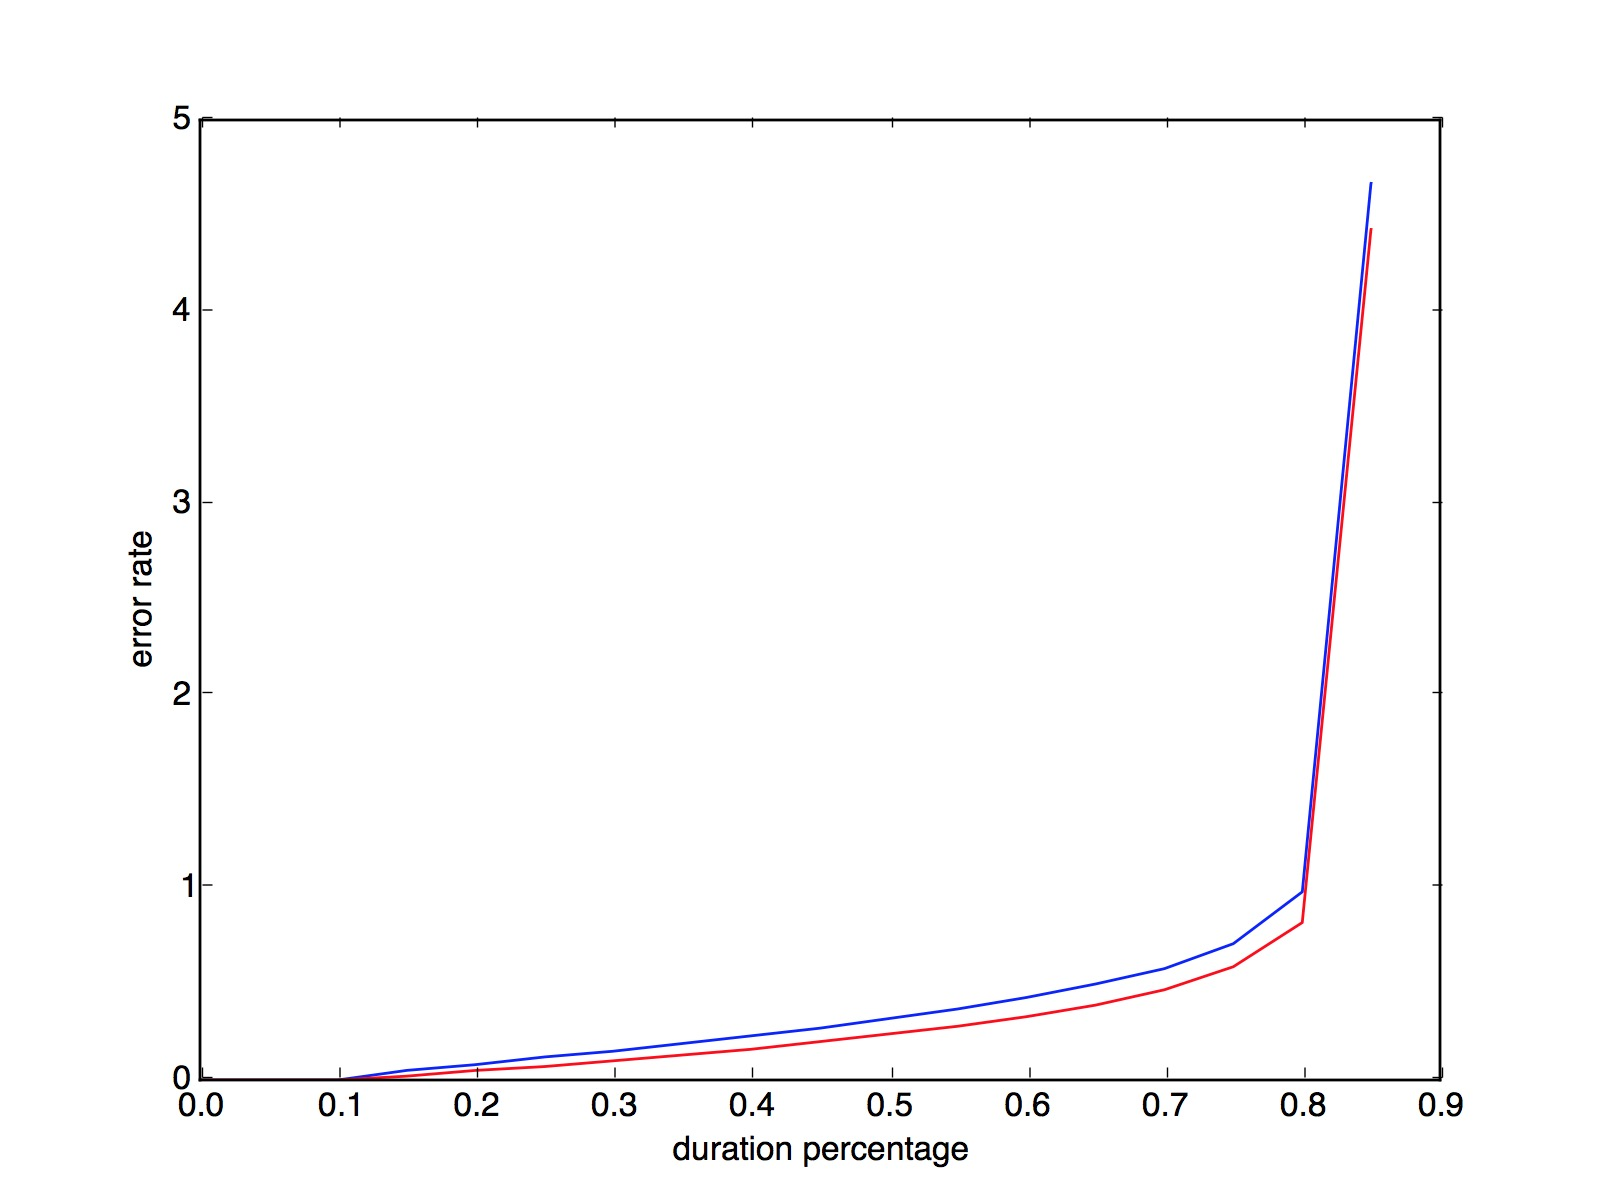
\includegraphics[scale=0.2]{wmerpmeram0s1} 
%\centering
%\end{figure}

%\begin{figure}
%\caption{Graph of PMER and WMER from transcription align, provided by MGB.}
%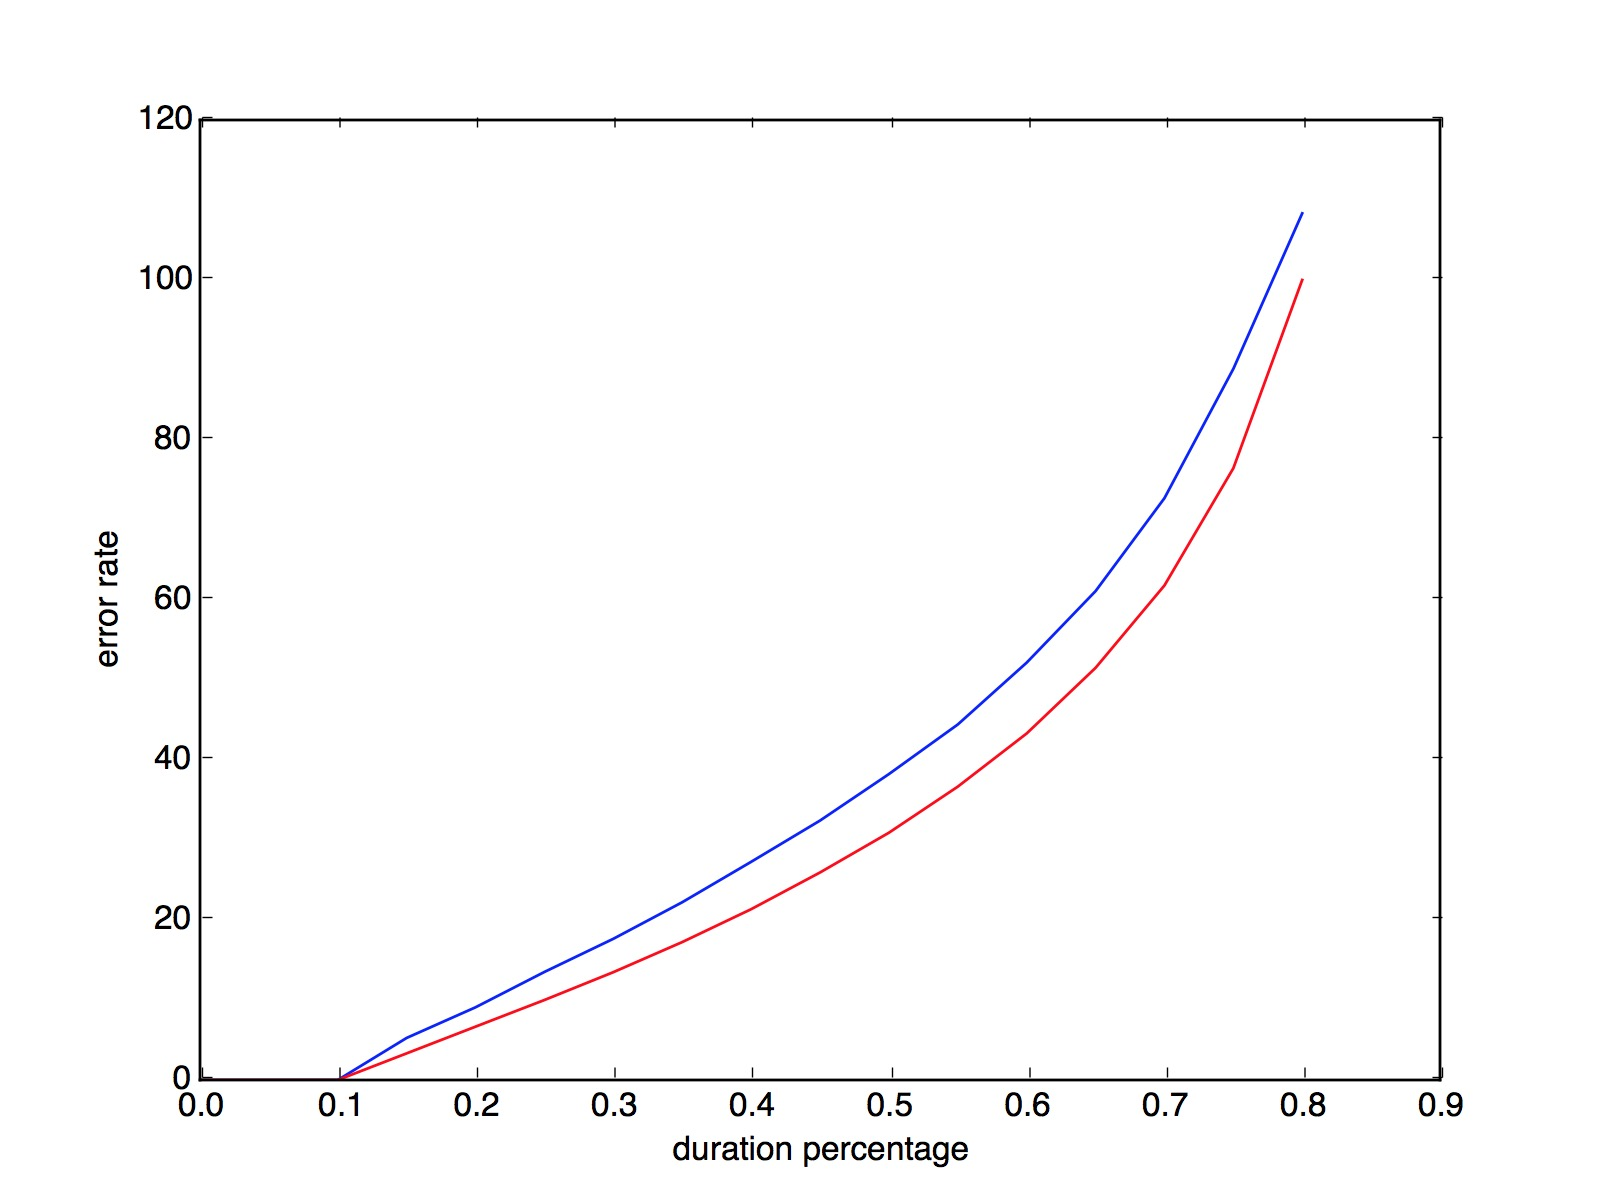
\includegraphics[scale=0.2]{wmerpmeram0align}
%\centering
%\end{figure}

%\subsubsection{Training acoustic model AM.100-v2}
%\begin{center}
%\begin{tabular}{ | c | c | c | c |  c |  }
%\hline
%\textbf{No.} & \textbf{Description} & \textbf{Result} & \textbf{execution time} & \textbf{extra info} \\ \hline \hline
%1 & GMM-V2\_decode &  & 2h 56m 41s & 20 hosts \\  \hline
%2 & TDNN-V2\_decode &  & 23h 52m 58s & 3 hosts \\  \hline
%\end{tabular}
%\end{center}


\section{Comparison}

Comparison between different speech recognizer:
\begin{center}
\label{wmerAM0s1}
\begin{tabular}{ | c | c | c |  c | c |  }
\hline
\textbf{No.} & \textbf{Acoustic model} & \textbf{Language Model}  &  \textbf{PER}  & \textbf{WER}  \\ \hline \hline
1 & TDNN.100  & LM.7weeks+subtitles.limited.1e-9 & 35.8  & 43.9 \\ 
& & Lexicon.7weeks+subtitles  & & \\ \hline


2 & TDNN.100-v1\_decode   & LM.7weeks+subtitles.limited.1e-9  & 34.3    & 42.3 \\
&  & Lexicon.7weeks+subtitles & & \\ \hline

3 & TDNN.100-v1   & LM.7weeks+subtitles.limited.1e-9  & 33.8   & 41.2 \\
&  & Lexicon.7weeks+subtitles & & \\ \hline


4 & TDNN.100-v2   & LM.7weeks+subtitles.limited.1e-9  & 33.3    & 40.5 \\
&  & Lexicon.7weeks+subtitles & & \\ \hline

5 & TDNN.100-v3   & LM.7weeks+subtitles.limited.1e-9  & 33.3    & 40.5 \\
&  & Lexicon.7weeks+subtitles & & \\ \hline
\end{tabular}
\end{center}


\begin{figure}
\caption{Average word duration}
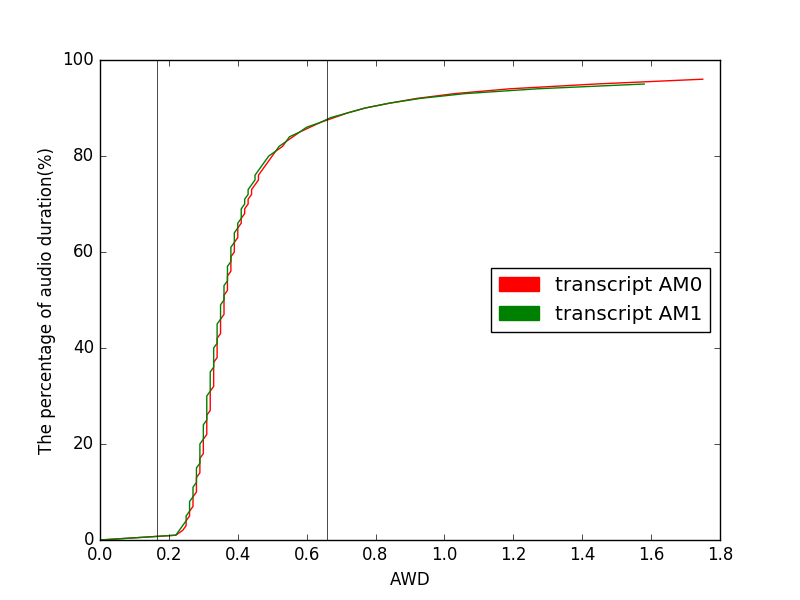
\includegraphics[scale=0.7]{awdLineChart}
\centering
\end{figure}

\begin{figure}
\caption{Phone match error rate}
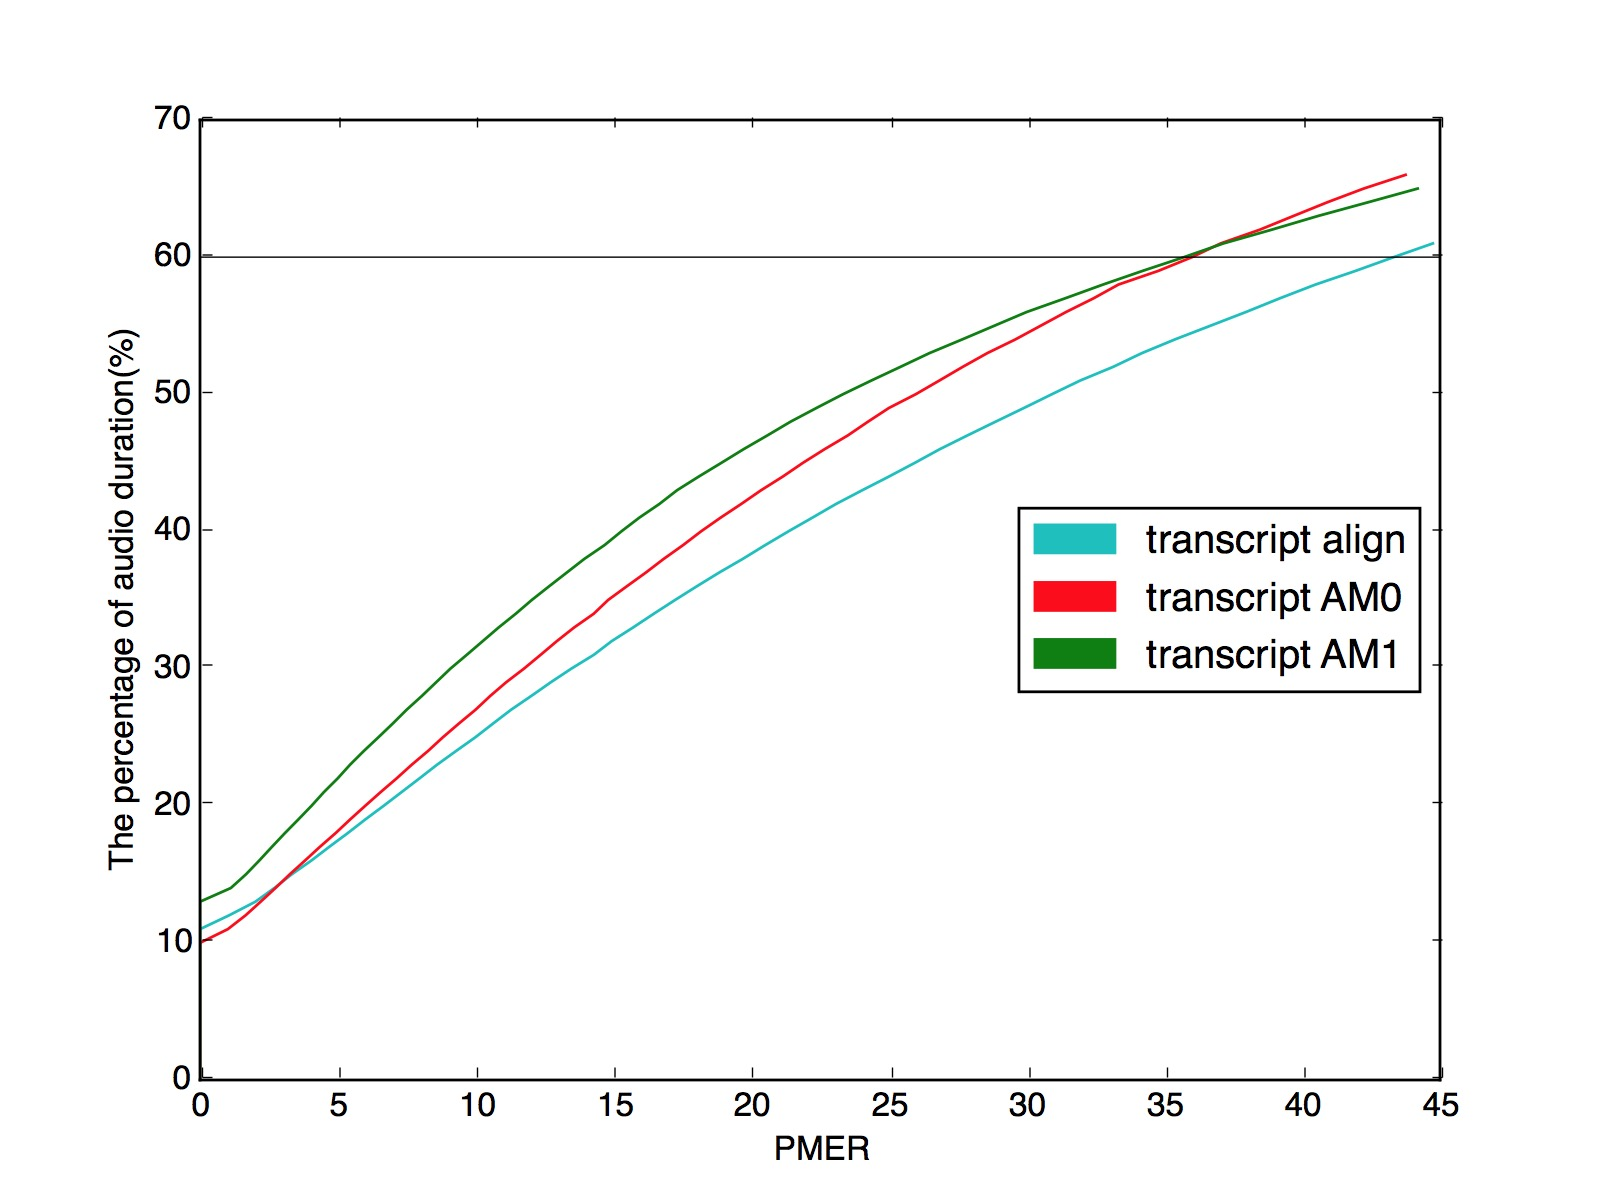
\includegraphics[scale=0.3]{pmerLineChart}
\centering
\end{figure}

\begin{figure}
\caption{Word match error rate}
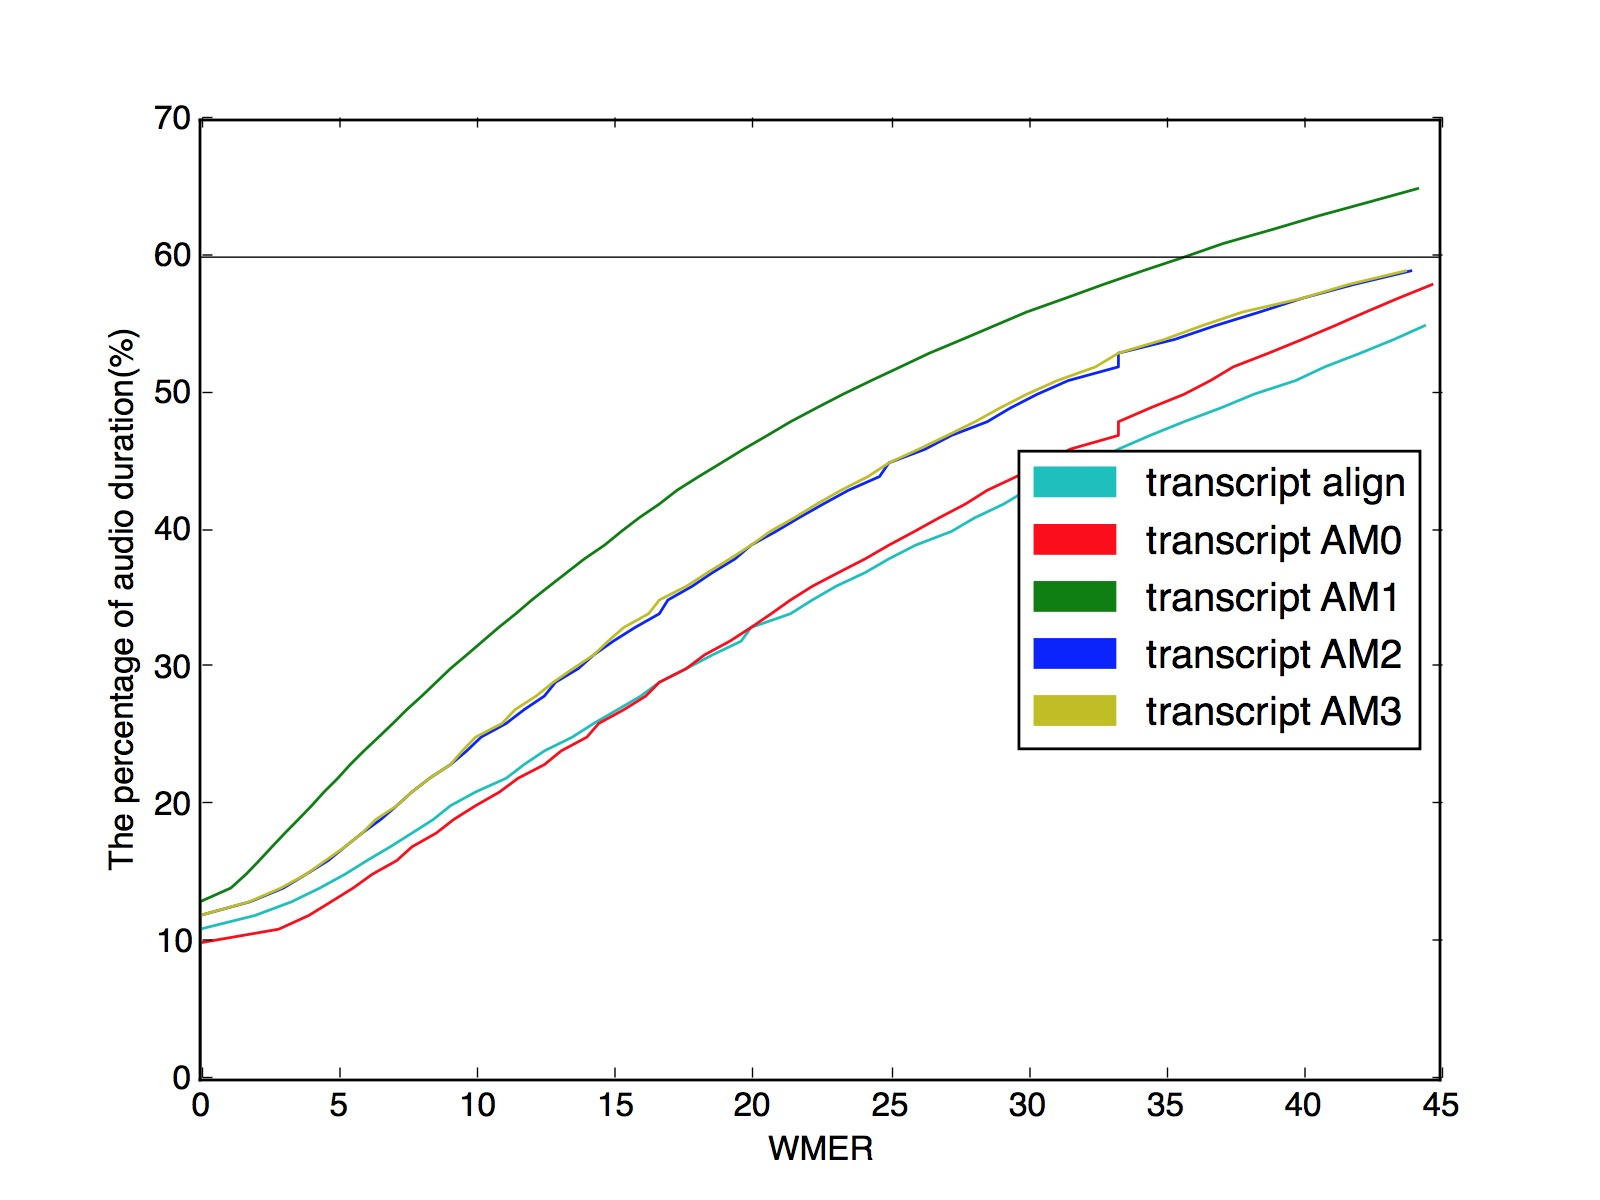
\includegraphics[scale=0.25]{wmerLineChart}
\centering
\end{figure}




%PER 32.2 | 9118 204786 | 75.0 10.0 15.0 7.2 32.2 82.7 | -1.058 | |
%WER 49.3 | 9118 64248 | 59.0 25.1 15.9 8.2 49.3 83.7 | -0.822 | |

%AM0_s1
%WMER
%[0, 0.05001182297101408, 0.1000055705823501, 0.15002999947778156, 0.20000377990423135, 0.250006911717846, 0.3000083202847346, 0.350008061797726, 0.4000080655439148, 0.45000218777410367, 0.5000070802963298, 0.5500076834326855, 0.6000113209817511, 0.6500022214898035, 0.7000031243212423, 0.7500004870045146, 0.8000498093227562, 0.8500152732106541]
%[0, 0.0, 0.0, 0.05, 0.08, 0.12, 0.15, 0.19, 0.23, 0.27, 0.32, 0.37, 0.43, 0.5, 0.58, 0.71, 0.98, 4.67]

%PMER
%[0, 0.05000255115439209, 0.10000343525488571, 0.15000458158857732, 0.20000319924500873, 0.2500218028172682, 0.3000072338900607, 0.3500012437345947, 0.4000032891535333, 0.45000364878763255, 0.5000033341077957, 0.5500060913025576, 0.6000314567451253, 0.6500026335705453, 0.700001251226977, 0.7500149847541436, 0.8000220313347739, 0.8500007005372576]
%[0, 0.0, 0.0, 0.02, 0.05, 0.07, 0.1, 0.13, 0.16, 0.2, 0.24, 0.28, 0.33, 0.39, 0.47, 0.59, 0.82, 4.43]

%Align
%WMER
%([0, 0.050002832118532126, 0.10000931677088468, 0.15000742869186362, 0.20000679558600154, 0.2500274408310134, 0.30000118379557716, 0.3500026485552931, 0.40000639849001596, 0.4500279240893308, 0.5000118004938804, 0.5500090133296115, 0.6000040159141051, 0.6500046752432919, 0.7000030681284111, 0.7500003184260248, 0.800006522114234], [0, 0.0, 0.0, 5.26, 9.09, 13.51, 17.65, 22.22, 27.27, 32.43, 38.24, 44.44, 52.17, 61.11, 72.73, 88.89, 108.33], 'b-'

%PMER
%[0, 0.05001950265750902, 0.10000225520549781, 0.15000134113549585, 0.20000690797165727, 0.25000294075800095, 0.30001437037921774, 0.35000064434442896, 0.40001250477732614, 0.45001977612927163, 0.5000107890229769, 0.5500005656744683, 0.60003347968693, 0.6500121301584764, 0.7000086499493287, 0.7500019667489803, 0.800000340903153], [0, 0.0, 0.0, 3.33, 6.67, 10.0, 13.48, 17.24, 21.35, 25.94, 30.91, 36.67, 43.32, 51.52, 61.82, 76.47, 100.0], 'r-'

 
\chapter{Implementation}

\section{Data set}
% cite it here
For this internship, we used TV broadcasts downloaded from the internet. 
\begin{itemize}
\item The audio files are taken from TV broadcasts. Total duration of audio is around 200 hours.
\item TV broadcast transcriptions(closed captions) of the audio files are provided. The closed captions are close to what the audio says, but not exactly the same as the speakers of the audio said. In addition to the closed captions from 200 hours TV broadcasts, we have the closed captions from 1600 hours of TV broadcasts as well.
\item 640 million words of TV subtitles are provided. In addition to that, the 640M subtitles are filtered to avoid overlap with the closed captions from the TV broadcasts.
\end{itemize} 

We prepared two data sets: training set and development set. The training dataset has a total duration of around 200 hours of audio. To evaluate our model, we have a development set. Some metadata are provided in our data, such as: speaker id of the transcript, genre of the show, date and time of the show, as well as television channel where the show was aired. In addition, each segment has start and end time when the segment was shown in the TV broadcast. All files in full training set have closed captions. In contrast, all files in development set have closed captions as well as manually annotated human transcription. The transcript is manually and carefully annotated by human. Thus, the transcript is believed to be the closest transcription spoken by speakers in audio files. 

Table \ref{tab:dataset} shows the statistics of the training set and the development set. The second column represents the number of TV shows in each genre; the third column represents the total duration of each genre. Lastly, the forth column(the last column) shows the total duration of speech when the speakers spoke in the audio.
\begin{center}
\label{tab:dataset}
\captionof{table}{Dataset duration}
\begin{tabular}{ | c | c | c | c | c |  }
\hline
No & Data set & \#shows & Duration(h) & Aligned speech (h) \\ \hline
1 & training set & 274 & 193  & 149 \\ \hline
2 & development set & 12 & 8 & 6 \\ \hline
\end{tabular}
\end{center}

 After obtaining 200 hours of data, a 100 hours subset was created by selecting one from two files from 200 training set. The 200 hours and 100 hours training set are named as train.200 and train.100 respectively. 

\begin{center}
\label{statisticstrain200}
\captionof{table}{Statistics of train.200 per genre}
\begin{tabular}{ | c | c | c | c|}
\hline
\textbf{Genre} & \textbf{\#shows}  & \textbf{Duration(h)} & Aligned speech(h) \\ \hline \hline
advice & 40 & 26 & 22 \\ \hline
children & 51 & 19 & 14 \\ \hline
comedy & 19 & 8 & 6 \\ \hline
competition & 30 & 21 & 16 \\ \hline
documentary & 29 & 22 & 14 \\ \hline
drama & 20 & 14 & 10 \\ \hline
events & 24 & 38 & 29 \\ \hline
news & 61 & 42 & 37 \\ \hline
\end{tabular}
\end{center}


%Table \ref{statisticstrain200} shows the statistics of each genre in the train.200 training set. 

\section{Experiment setup}
In this section, we explained how we did the experiments. First, we elaborated how to build language models,  then the acoustic model, and lastly how to decode the data set for the data selection and the model evaluation.

\subsection{Language model}
\subsubsection{Library: SRILM}
SRILM is a toolkit which comprises of a collection of executable programs, which are written in C++, for creating and applying statistical language models for speech recognition and other natural language applications \cite{Stolcke02srilm}. SRILM supports several operations for language model(LM), such as: creating a language model from a text corpus, interpolating several language models into one, pruning a language model, and estimate perplexity of a language model against the test corpus. 

The below code is an example how to make a 4-gram language model with input from $CORPUS$ and interpolated with Kneser-ney interpolation \cite{KneserNey1993}. The syntax is pretty straightforward and easy to understand. The resulted language model will be written in arpa language model format.
\begin{verbatim}
ngram-count -order 4 -kndiscount -interpolate -sort -text CORPUS -lm LM
\end{verbatim}

\subsubsection{Implementation}
\label{3LM}
This internship experimented with three different kinds of language model for speech recognition. All language models are based on four gram language model. We will describe language model from the most constraint to the less constraint
\begin{enumerate}
\item LM.200 \\
This language model, named as LM.200, was produced from the closed captions of 200 hours training set(train.200). LM.200 was pruned by $10^{-9}$. Pruning means deleting 4 gram sequences which are less than $10^{-9}$.  LM.200 was used for the baseline speech recognizer to select the "good" subset of data.

\begin{center}
\captionof{table}{Statistics of LM.200}
\begin{tabular}{ | c | c | c | }
\hline
\textbf{No.} & \textbf{File}  & \textbf{Information} \\ \hline \hline
1 & word.200 & 33,914 words \\  \hline
2 & LM.200 & uni-gram=33916 \\ 
 & & bi-gram=402299 \\ 
& & tri-gram=111868 \\  
& & 4-gram=64801 \\  \hline
3 & LM.200.1e-9 & ngram 1=33916 \\  
 & & ngram 2=402299 \\  
& & ngram 3=98566 \\  
& & ngram 4=51215 \\  \hline
\end{tabular}
\end{center}

\item LM.7weeks+subtitles.limited.1e-9 \\
A language model was generated from the closed captions of 1600 hours transcription(7weeks TV broadcast closed captions) and interpolated with a language model from the big TV subtitles with ratio 0.9/0.1. The language model was limited by top 160,000 frequent word list and pruned by $10^{-9}$ resulting in LM.7weeks+subtitles.limited.1e-9.  The language model and together with an acoustic model and a lexicon was utilized to compute error rate of the development set.

\begin{center}
\begin{tabular}{ | c | c | c | }
\hline
\textbf{No.} & \textbf{File}  & \textbf{Information} \\ \hline \hline
1 & word.160k & 160,000 words \\  \hline
2 & LM.7weeks & ngram 1=91836 \\
 & & ngram 2=1817881 \\
 & & ngram 3=980925 \\
 & & ngram 4=847736 \\  \hline
3 & LM.subtitles & ngram 1=756644 \\
 & & ngram 2=27144330 \\
 & & ngram 3=37162518 \\
 & & ngram 4=57912280 \\ \hline
4 & LM.7weeks+subtitles & ngram 1=768522 \\
 & & ngram 2=27441072 \\
 & & ngram 3=37312673 \\
 & & ngram 4=58183256 \\ \hline
5 & LM.7weeks+subtitles.limited & ngram 1=160002 \\
 & & ngram 2=24926818 \\
 & & ngram 3=32102763 \\
 & & ngram 4=44253079 \\ \hline
5 & LM.7weeks+subtitles.limited.1e-9 &ngram  1= 160002 \\
 & & ngram  2=   5251197 \\
 & & ngram  3=   3876171 \\
 & & ngram  4=   2453067 \\ \hline
\end{tabular}
\end{center}

\item LM.genres \\
Eight language models were generated from each genre(LM.documentary, LM.news, LM.events, LM.drama, LM.competition, LM.comedy, LM.children, and LM.advice). Then, each language model was interpolated with the big subtitle LM with  ratio 0.9/0.1, limited by the top 160,000 word list, and pruned by $10^{-9}$ threshold. The language model was used in the new proposed algorithm only.

\begin{center}
\begin{tabular}{ | c | c | c | }
\hline
\textbf{No.} & \textbf{File}  & \textbf{Information} \\ \hline \hline
1 & LM.documentary & ngram 1=37542
ngram 2=437631
ngram 3=135632 \\
& & ngram 4=90381   \\ \hline
2 & LM.news & ngram 1=44588
ngram 2=661625
ngram 3=305473 \\
& & ngram 4=255125  \\ \hline
3 & LM.events & ngram 1=23717
ngram 2=306938
ngram 3=125934 \\
& & ngram 4=95203  \\ \hline
4 & LM.drama & ngram 1=21345
ngram 2=202078
ngram 3=60920 \\
& & ngram 4=40073  \\ \hline
5 & LM.competition &  ngram 1=33269
ngram 2=385257
ngram 3=124584 \\
& & ngram 4=89642 \\ \hline
6 & LM.comedy & ngram 1=20180
ngram 2=165073
ngram 3=39353 \\
& & ngram 4=23877  \\ \hline
7 & LM.children &  ngram 1=27029
ngram 2=287141
ngram 3=84063 \\
& & ngram 4=57851 \\ \hline
8 & LM.advice & ngram 1=30545
ngram 2=397766
ngram 3=154416 \\
& & ngram 4=108794  \\ \hline
\end{tabular}
\end{center}

\end{enumerate}

To build language models we mentioned before, we utilized SRILM. In addition to building language models, SRILM is able to interpolate several language models, limit vocabularies of a language models, prune a language model by a threshold, and many more.


\subsection{Acoustic model}
\subsubsection{Library: Kaldi}
Kaldi is a toolkit, written in C++, which comprises several tools which are useful to experiment and build a speech recognition system \cite{PoveyASRU2011}. Kaldi supports several operations to build a speech recognition system, such as: extracting feature vectors, acoustic modeling, training acoustic models, and creating decoding graph as well as decoding audio inputs into lattices. Kaldi provides several features, such as:
\begin{itemize}
\item It support finite state transducer(FST), which is based on OpenFST library. The FST is used to build a decoding graph with the inputs of acoustic model, language model, and lexicon.
\item It is extensible and provides complete recipes. Kaldi gives many recipes to build acoustic model, such as: gaussian mixture model, deep neural network, etc.
\item It supports linear algebra and utilizes the standard linear algebra library: BLAS and LAPACK.
\item It has been tested thoroughly to ensure the quality of the library.
\end{itemize}

\subsubsection{Acoustic model implementation}
%GMM
Before training the DNN acoustic model, GMM-HMM must be trained first. GMM-HMM is able to perform force alignment on the flat start(without phoneme-to-audio alignment). The labeling of each acoustic input is compulsory to train the TDNN acoustic model. 

We utilized TED-LIUM's recipe(nnet3 in Kaldi) to train the TDNN acoustic model. The feature vector is extracted with MFCC, consisting of 40 feature values. The TDNN architecture has 6 hidden layers, where each hidden unit  utilizes rectified linear unit(RELU) activation function. The TDNN outputs around 9000 output nodes with softmax activation function. Moreover, the TDNN architecture is implemented by leveraging the subsampling technique. Table shows the parameters and subsampling splice configuration we used in the architecture.

\begin{center}
\captionof{table}{Parameters of  theTDNN acoustic model}
\label{TDNNparams}
\begin{tabular}{ | c | c | }
\hline
\textbf{Parameter} & \textbf{Method}  \\  \hline \hline
initial learning rate & 0.0015 \\
final learning rate & 0.00015 \\ \hline
mini batch size & 512 \\ \hline
epoch & 3 \\ \hline
subsampling splice & \\
layer 1 & $t-2,t-1,t,t+1,t+2$ \\
layer 2 & $t-1,t+2$ \\
layer 3 & $t-3,t+3$ \\
layer 4 & $t-7,t+2$ \\
layer 5 & $t-3,t+3$ \\
layer 6 & $t$ \\  \hline
\end{tabular}
\end{center}
% features
% architecture

% hyperparameters
% -splice
% -learning rate
% -training

\subsection{Recognition}
The last step after training an acoustic model and building a language model is to recognize a data set. The recognition is useful for data selection(computing the new word error rate as well as phone error rate ) and evaluate how good our data selection is. In overall, the recognition(or decoding) process works as following:
\begin{enumerate}
\item Create a decoding graph from an acoustic model, a language model, and a lexicon. In Kaldi's implementation, it transforms the  acoustic model, the language model, and the lexicon into a weighted finite state transducer(WFST).
\item Decode the dataset by using the WFST. In Kaldi, the decoding process will result in a lattice. Lattice is a decoding graph which represents some variants of the recognition. Providing only one best recognition is not practical; thus lattice is the way to represent the recognition/decoding result. 
\item Compute the best path of word or phone in the lattice and calculate the WER as well as PER. Kaldi produces two ctm files(word and phone ctm files) which are the best decoding results which the algorithm can obtain. The ctm file consists of words(or phone) in the transcription with its start and end time relative to the audio. By utilizing sclite, the ctm file(the hypothesized word/phone from the ASR) is compared with the transcriptions(the closed captions or the detailed transcription). Then, the code matches and computes the minimum edit distance to calculate the error rate.
\end{enumerate}

\subsubsection{Data Selection}
To select the good data for the next iteration, the new matched word and phone error rate must be generated from the training set. By running the recognition steps(as explained above) on the training set and comparing the decoding result with the closed captions, a file(the file with the extension of ".prf") is generated. The file contains the number of insertion, deletion, and substitution. By using the error rate equation as bellow, the new matched error rate(WMER and PMER) are computed. 

Firstly, the segments are sorted based on the new PMER. Secondly, choose the top 100 hour segments based on the PMER. These selected segments are used for the next iteration. 

\subsubsection{Evaluation}
To evaluate how good our data selection is, we need to evaluate the automatic speech recognizer(especially the acoustic model). In every iteration, we train an acoustic model; furthermore, the acoustic model and together with the language model(LM.7weeks+subtitles.limited.1e-9) as well as the lexicon, we recognize the development set. After decoding and computing WER of development set, we compare the WER with the previous iteration. If the new WER is lower, we can continue the iteration; otherwise, stop the iteration. 

\subsubsection{Experiments}

\section{Experiment resources}
To run our experiment, we utilized grid 5000 server cluster. Grid 5000 is a computing cluster with a focus on parallel and distributed computing \cite{Grid5000}. It has several key features:
\begin{itemize}
\item It provides a large amount of resources, over 1000 nodes, and massive volume of hard disk.
\item The experiment is highly configurable where we can specify number of nodes and the criteria of the nodes which we will use.
\item We can do advanced monitoring of memory usage, cpu usage, and the log of our experiment which later be used to analyze the experiment.
\end{itemize}

The following is the description of resources which we leveraged for this internship based on the tasks:
\begin{enumerate}
\item Train acoustic models: 1 computer with GPU and 8 computers without GPU. At least one computer with GPU is compulsory because we can harness GPU to parallelization the computation of DNN training. 
\item Create decoding graph only needs one computer because the Kaldi recipe does not need parallelization for this process.
\item Decoding the ASR leverages 20 computers. Usually one computer can recognize one hour of audio within one hour. Therefore, the more computer we use, the faster the decoding process will be. 
\item Lastly, the error rate computation and data selection process only utilizes one computer. 
\end{enumerate}
% server
% exectution time

 
\chapter{Experiment results}

%\textbf{Insert time and perpelexity here.}

\section{Baseline model}

\subsection{Acoustic model AM.200 and Language Model Version 1 (LM.200.1e-9)}
\label{amv0s1}


Calculating PMER and WMER for each segment by utilizing AM.200 and LM.200.1e-9:
\begin{enumerate}
\item GMM(GMM.200): GMM is trained by using the 200 hours data
\item TDNN(TDNN.200): the result of GMM training(GMM.200) is utilized to build a TDNN(time delay neural network). 
\item TDNN graph creation \\
The language model used is the LM.200.1e-9 and  the acoustic model is  TDNN.200; furthermore, the dictionary used(Lexicon.200) is the modification of the library provided by MGB(Lexicon.MGB). Words in Lexicon.MGB which do not exist in word.200 are removed from Lexicon.200.
%\item TDNN development set recognition \\
%The development set is files from dev.short, which contains 8 hours of audio. The development set is recognized by leveraging the graph created in the previous step.
\item TDNN 200 hours of training data recognition \\
We need to recognize 200 hours data to calculate PMER, WMER, and AWD. This data will be used for data selection of the next iteration.
\item Sclite score PMER and WMER \\
Use the lattice and graph(produced at step 5 and 3 respectively) to calculate overall PMER and WMER. However, the decoding program does not provide PMER, WMER, and AWD for each segment. Fortunately, the program generates prf file which contains number of correction, insertion, deletion, and substitution for each segment. Two prf files exist after decoding:(ctm\_words.filt.filt.prf contains word match error rate and ctm\_phones.filt.filt.prf contains phone match error rate). From there, we are able to calculate  PMER, WMER, and AWD of each segments.  For the development set, we only need to know the overall PER and WER. In contrast, training set recognition needs PMER, WMER, and AWD for each segment. 

\end{enumerate}


version AM0
% table
\begin{center}
\begin{tabular}{ | c | c | c | c |  c |  }
\hline
\textbf{No.} & \textbf{Description} & \textbf{Result} & \textbf{execution time} & \textbf{extra info} \\ \hline \hline
1 & GMM.100  &  & 3h 30m & 20 hosts \\  \hline
%/talc2/multispeech/calcul/users/jkarsten/mgb/recipe/tools/baseline/baseline1_backup/gmm
%1.1 & GMM decoding & 57.2\% WER  & 3h 36m 47s & 20 hosts, 4 cores \\  \hline \hline
%2 & AM.200 training. &  & 38h 30m 31s & 3 nodes \\  

2 & TDNN.100 training: & & 17h 7m & 3 GPU hosts \\ 
 & LM.200.1e-9,  GMM.100, Lexicon.200 &  & & \\ \hline
 %/talc2/multispeech/calcul/users/jkarsten/mgb/recipe/tools/baseline/baseline1_backup/tdnn
 
3 & Create a graph from TDNN.200,  &  & 6m & 1 host \\  
 & LM.200.1e-9, Lexicon.200  & & & \\ \hline
%/talc2/multispeech/calcul/users/jkarsten/mgb/recipe/tools/modifASR/tdnn_s1/graph_creation_from_arpaLM

4 & Create a graph from TDNN.200,  &   & 4h 49m & 1 host \\  
 & LM.7weeks+subtitles.1e-9, Lexicon.200  & & & \\ \hline

%4 & AM.200 recognized dev.short &  & 2h 58m 58s   & 20 hosts  \\  \hline
5 & TDNN.100 recognized train.200 &  & 16h 6m & 20 hosts \\  \hline 
 %/talc2/multispeech/calcul/users/jkarsten/mgb/recipe/tools/modifASR/tdnn_s1/recognition_with_scoring/decode_res_train_200_fst+merall_mgb2015.wordList.4gm.kn.arpa.gz.1e-9.arpa_4thr

6 & TDNN.100 \& LM.7weeks+subtitles.1e-9 & WER 43.9\%   & 45m & 20 hosts \\  
&  recognized dev.short & PER 35.8\% & & \\ \hline
%5 & Calculate Overall PMER & 24.8 \% PMER   & 5h 5m 51s & 1 host \\  \
 %& and WMER of train.200  & 32.4 \% WMER & & \\ \hline
%5.1 &  Calculate PMER and WMER & & 20m 22s & 1 host \\  
 %&  per segment of step 6 & & &  \\  \hline
%/talc2/multispeech/calcul/users/jkarsten/mgb/recipe/tools/modifASR/tdnn_s1/sclite_score_pmer_and_wmer
% /talc2/multispeech/calcul/users/jkarsten/mgb/recipe/tools/modifASR/tdnn_s1/calculate_pmer_wmer_per_segments

%6 & Calculate PER  &  32.5 \% PER  & 1h 10m 57s   & 1 host \\  \
% & PMER, WMER calculation  &   48.7\% WER   & & \\ \hline
\end{tabular}
\end{center}


%%%%%%%%%%%%%%%%%%%%%%%%%%%%%%%%%%%%%%%%
% table
version AM1
\begin{center}
\begin{tabular}{ | c | c | c | c |  c |  }
\hline
\textbf{No.} & \textbf{Description} & \textbf{Result} & \textbf{execution time} & \textbf{extra info} \\ \hline \hline
1 & GMM.100  &  & 4h 7m & 20 hosts \\  \hline

2 & TDNN.100 training: & & 20h 1m & 3 GPU hosts \\ 
 & LM.200.1e-9,  GMM.100, Lexicon.200 &  & & \\ \hline
 
3 & Create a graph from TDNN.200,  &  & 5m & 1 host \\  
 & LM.200.1e-9, Lexicon.200  & & & \\ \hline
 
4 & Create a graph from TDNN.200,  &   & 3h 7m & 1 host \\  
 & LM.7weeks+subtitles.1e-9, Lexicon.200  & & & \\ \hline

5 & TDNN.100 recognized train.200 &  & 14h 18m & 20 hosts \\  \hline 

6 & TDNN.100 \& LM.7weeks+subtitles.1e-9 & WER 41.2\%   & 46m & 20 hosts \\  
&  recognized dev.short & PER 33.8\% & & \\ \hline
\end{tabular}
\end{center}

%%%%%%%%%%%%%%%%%%%%%%%%%%%%%%%%%%%%%%%%
version AM2
\begin{center}
\begin{tabular}{ | c | c | c | c |  c |  }
\hline
\textbf{No.} & \textbf{Description} & \textbf{Result} & \textbf{execution time} & \textbf{extra info} \\ \hline \hline
1 & GMM.100  &  & 3h 3m & 20 hosts \\  \hline

2 & TDNN.100 training: & & 23h 58m & 3 GPU hosts \\ 
 & LM.200.1e-9,  GMM.100, Lexicon.200 &  & & \\ \hline
 
3 & Create a graph from TDNN.200,  &  & 5m & 1 host \\  
 & LM.200.1e-9, Lexicon.200  & & & \\ \hline
 
4 & Create a graph from TDNN.200,  &   & 3h 13m & 1 host \\  
 & LM.7weeks+subtitles.1e-9, Lexicon.200  & & & \\ \hline

5 & TDNN.100 recognized train.200 &  & 15h 51m & 20 hosts \\  \hline 

6 & TDNN.100 \& LM.7weeks+subtitles.1e-9 & WER 40.5\%   & 36m & 20 hosts \\  
&  recognized dev.short & PER 33.3\% & & \\ \hline
\end{tabular}
\end{center}


%%%%%%%%%%%%%%%%%%%%%%%%%%%%%%%%%%%%%%%%
version AM2
\begin{center}
\begin{tabular}{ | c | c | c | c |  c |  }
\hline
\textbf{No.} & \textbf{Description} & \textbf{Result} & \textbf{execution time} & \textbf{extra info} \\ \hline \hline
1 & GMM.100  &  & 3h 3m & 20 hosts \\  \hline

2 & TDNN.100 training: & & 25h 27m & 3 GPU hosts \\ 
 & LM.200.1e-9,  GMM.100, Lexicon.200 &  & & \\ \hline
 
3 & Create a graph from TDNN.200,  &  & 7m & 1 host \\  
 & LM.200.1e-9, Lexicon.200  & & & \\ \hline
 
4 & Create a graph from TDNN.200,  &   & 4h 49m & 1 host \\  
 & LM.7weeks+subtitles.1e-9, Lexicon.200  & & & \\ \hline

5 & Create a graph from TDNN.200,  &   & 2h 1m each genre & 1 host \\  
 & LM.genres.1e-9, Lexicon.200  & & & \\ \hline

6 & TDNN.100 recognized train.200 &  & 15h 52m & 20 hosts \\  \hline 

7 & TDNN.100 \& LM.7weeks+subtitles.1e-9 & WER 40.5\%   & 38m & 20 hosts \\  
&  recognized dev.short & PER 33.3\% & & \\ \hline
\end{tabular}
\end{center}



%\subsection{Acoustic model AM.200 and Language Model LM.7weeks+subtitles.limited.1e-9}
% table
%\begin{center}
%\begin{tabular}{ | c | c | c | c |  c |  }
%\hline
%\textbf{No.} & \textbf{Description} & \textbf{Result} & \textbf{execution time} & \textbf{extra info} \\ \hline \hline
%3 & Create a graph from TDNN.200,  &  & 3h 12m 25s & 1 host \\   
% & LM.7weeks+subtitles.limited.1e-9,   & & & \\ 
% & Lexicon.7weeks+subtitles & & & \\ \hline
 %/talc2/multispeech/calcul/users/jkarsten/mgb/recipe/tools/modifASR/tdnn_s2/graph_creation_from_arpaLM


%4 & TDNN.200 &  & 1h 10m 59s & 20 hosts \\  
% & recognized dev.short & & & \\ \hline
% /talc2/multispeech/calcul/users/jkarsten/mgb/recipe/tools/modifASR/tdnn_s2/recognition_human/recognition_with_scoring_human


 %5 & TDNN.200 recognized &  & 10h 9m 35s & 20 hosts \\  
 %& train.200 & & & \\ \hline  
 %/talc2/multispeech/calcul/users/jkarsten/mgb/recipe/tools/modifASR/tdnn_s2/recognition_with_scoring
 
% 6 & TDNN AM.200 dev short & 31.8\% PER  & 4h 58m 26s & 1 hosts \\  
% & PMER, WMER calculation & 49.5\% WER & & \\ \hline
% 6.1 & TDNN AM-V0 train 200 & 26.4\% PMER & 4h 58m 26s & 1 hosts \\  
% & PMER, WMER calculation & 39.7\% WMER  & & \\ \hline
% 6.2 & Calculate PMER, WMER &  &  & 1 hosts \\  
 %& AWD per segment &  & & \\ \hline \hline
%\end{tabular}
%\end{center}


\subsection{Acoustic model(AM.200) and Language Model version 3(LM.genres)}


\subsection{Acoustic model AM.100-v1 and Language Model version 1 (LM.200.1e-9)}
% table
\subsubsection{100 hours selection(100-v1)}
How to select 100 hours subset of data for baseline model v1:
Section \ref{amv0s1}  calculates PMER, WMER, and AWD for each segments. Consequently, we can extract segments(of 200 hours transcriptions) which satisfy $0.165 \le AWD \le 0.66$. In the other word, the segments which does not satisfy are removed. Then, segments are sorted based on their PMER in ascending. We can deduce PMER threshold  and its total duration by sorting PMER as presented in the following table:  
\begin{center}
\label{pmerAM0s1}
\begin{tabular}{ | c | c | c | }
\hline
\textbf{PMER} & \textbf{Total duration} & \textbf{Percentage of total segment duration}  \\ \hline \hline
0.0 & 14.83 h & 10\% \\ \hline
5 & 29.66 h & 20\% \\ \hline
10 & 44.49 h & 30\% \\ \hline
16 & 59.32 h & 40\% \\ \hline
24 &  74.15 h & 50\% \\ \hline
33 & 88.98 h & 60\% \\ \hline
47 & 103.81 h & 70\% \\ \hline
82 & 118.64 h & 80\% \\ \hline
\end{tabular}
\end{center}


%PMER: 0.0; duration: 53389.43; percentage: 0.100003435255
%PMER: 0.05; duration: 106776.9; percentage: 0.200003199245
%PMER: 0.1; duration: 160166.65; percentage: 0.30000723389
%PMER: 0.16; duration: 213552.14; percentage: 0.400003289154
%PMER: 0.24; duration: 266939.76; percentage: 0.500003334108
%PMER: 0.33; duration: 320342.37; percentage: 0.600031456745
%PMER: 0.47; duration: 373713.84; percentage: 0.700001251227
%PMER: 0.82; duration: 427112.53; percentage: 0.800022031335

The Table \ref{pmerAM0s1} shows that 60\% of data has 33\% PMER with total duration of 88.98 hours of audio. From the table, we conclude that threshold 33 is selected as the threshold to select data for the next iteration.

\begin{center}
\label{wmerAM0s1}
\begin{tabular}{ | c | c | c | }
\hline
\textbf{WMER} & \textbf{Total duration} & \textbf{Percentage of total segment duration}  \\ \hline \hline
0.0 & 14.83 h & 10\% \\ \hline
8 & 29.66 h & 20\% \\ \hline
15 & 44.49 h & 30\% \\ \hline
23 & 59.32 h & 40\% \\ \hline
32 &  74.15 h & 50\% \\ \hline
43 & 88.98 h & 60\% \\ \hline
58 & 103.81 h & 70\% \\ \hline
98 & 118.64 h & 80\% \\ \hline
\end{tabular}
\end{center}

\subsubsection{Training Acoustic model AM.100-v1}



%\begin{center}
%\begin{tabular}{ | c | c | c | c |  c |  }
%\hline
%\textbf{No.} & \textbf{Description} & \textbf{Result} & \textbf{execution time} & \textbf{extra info} \\ \hline \hline
%1 & GMM.100-v1 &  & 3h 28m 43s & 20 hosts \\  \hline
%2 & TDNN.100-v1 &  & 26h 5m 3s & 3 hosts \\  \hline
%3 & GMM.100-v1\_decode &  & 2h 51m 4s & 20 hosts \\  \hline
%4 & TDNN.100-v1\_decode &  & 24h 30m 31s & 3 hosts \\  \hline
%\end{tabular}
%\end{center}


\subsection{The Second Acoustic model(AM.100-v2) and Language Model version 1 (LM.200.1e-9)}


%\begin{figure}
%\caption{Graph of PMER and WMER produced transcription AM-V0 and LM s1. The red line represents PMER, while the blue line represents WMER.}
%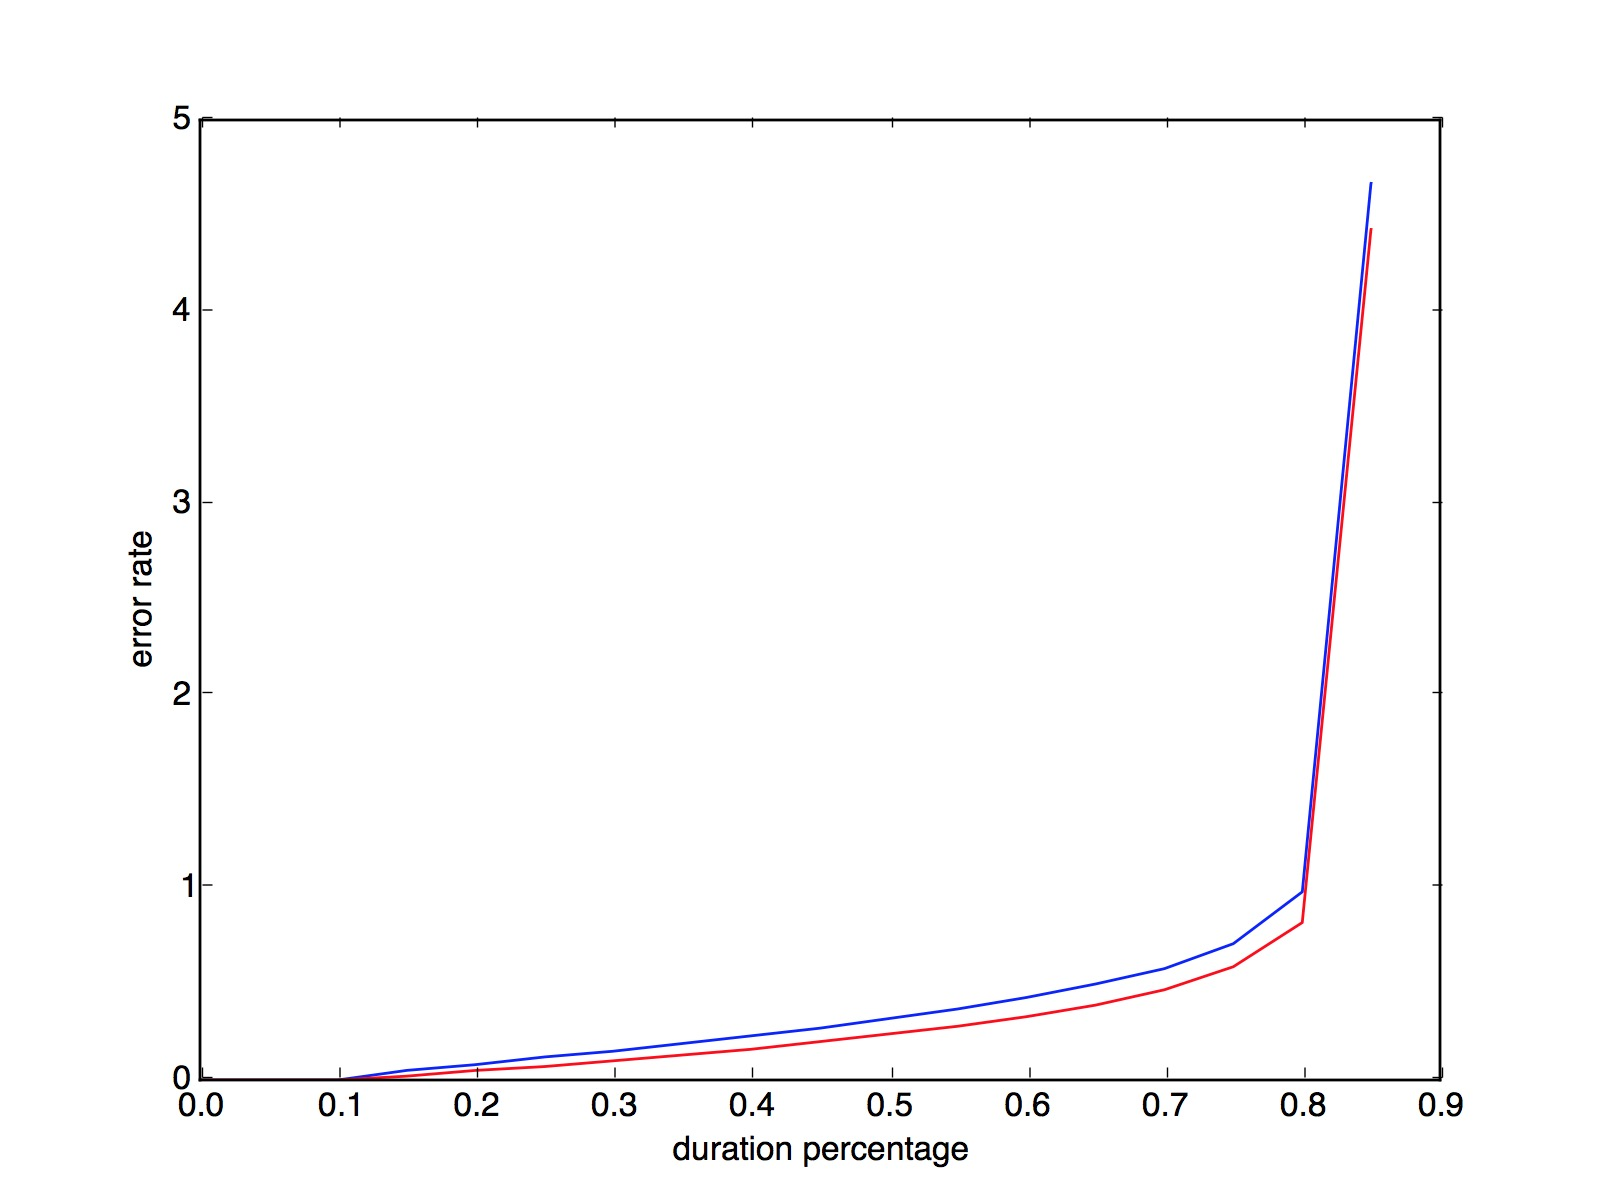
\includegraphics[scale=0.2]{wmerpmeram0s1} 
%\centering
%\end{figure}

%\begin{figure}
%\caption{Graph of PMER and WMER from transcription align, provided by MGB.}
%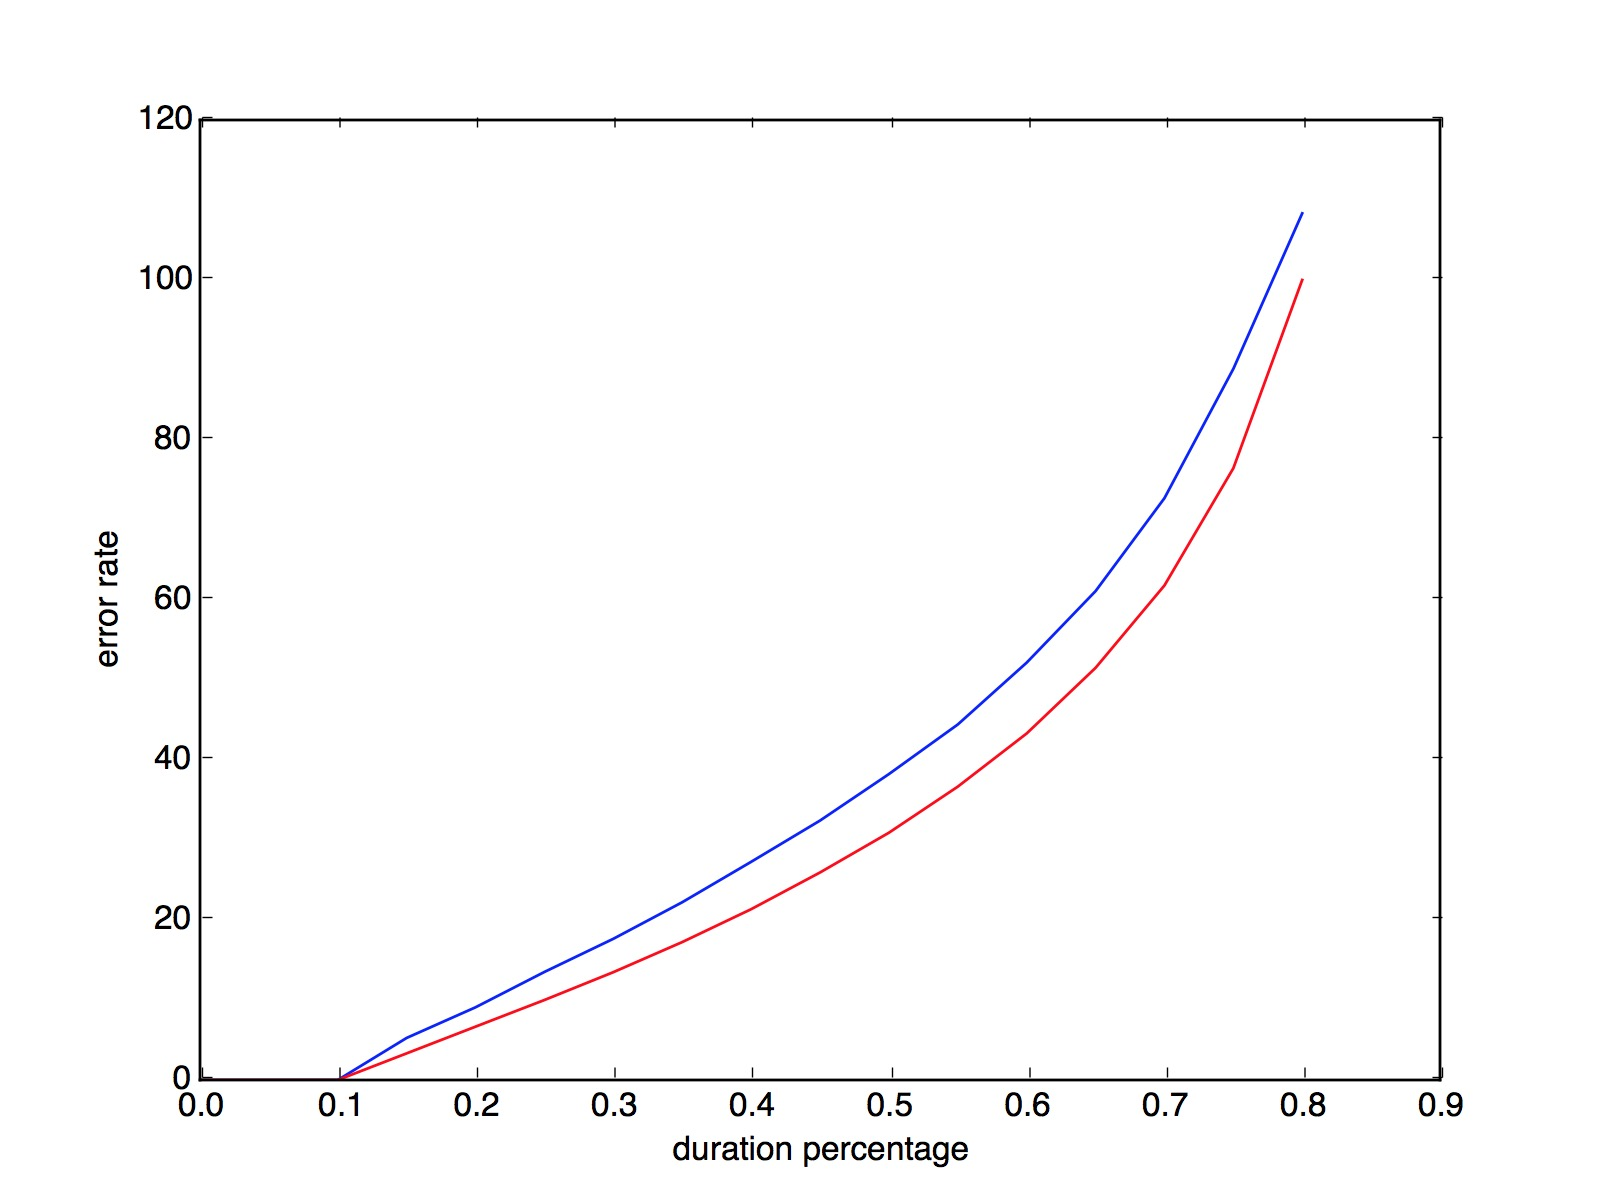
\includegraphics[scale=0.2]{wmerpmeram0align}
%\centering
%\end{figure}

%\subsubsection{Training acoustic model AM.100-v2}
%\begin{center}
%\begin{tabular}{ | c | c | c | c |  c |  }
%\hline
%\textbf{No.} & \textbf{Description} & \textbf{Result} & \textbf{execution time} & \textbf{extra info} \\ \hline \hline
%1 & GMM-V2\_decode &  & 2h 56m 41s & 20 hosts \\  \hline
%2 & TDNN-V2\_decode &  & 23h 52m 58s & 3 hosts \\  \hline
%\end{tabular}
%\end{center}


\section{Comparison}

Comparison between different speech recognizer:
\begin{center}
\label{wmerAM0s1}
\begin{tabular}{ | c | c | c |  c | c |  }
\hline
\textbf{No.} & \textbf{Acoustic model} & \textbf{Language Model}  &  \textbf{PER}  & \textbf{WER}  \\ \hline \hline
1 & TDNN.100  & LM.7weeks+subtitles.limited.1e-9 & 35.8  & 43.9 \\ 
& & Lexicon.7weeks+subtitles  & & \\ \hline


2 & TDNN.100-v1\_decode   & LM.7weeks+subtitles.limited.1e-9  & 34.3    & 42.3 \\
&  & Lexicon.7weeks+subtitles & & \\ \hline

3 & TDNN.100-v1   & LM.7weeks+subtitles.limited.1e-9  & 33.8   & 41.2 \\
&  & Lexicon.7weeks+subtitles & & \\ \hline


4 & TDNN.100-v2   & LM.7weeks+subtitles.limited.1e-9  & 33.3    & 40.5 \\
&  & Lexicon.7weeks+subtitles & & \\ \hline

5 & TDNN.100-v3   & LM.7weeks+subtitles.limited.1e-9  & 33.3    & 40.5 \\
&  & Lexicon.7weeks+subtitles & & \\ \hline
\end{tabular}
\end{center}


\begin{figure}
\caption{Average word duration}
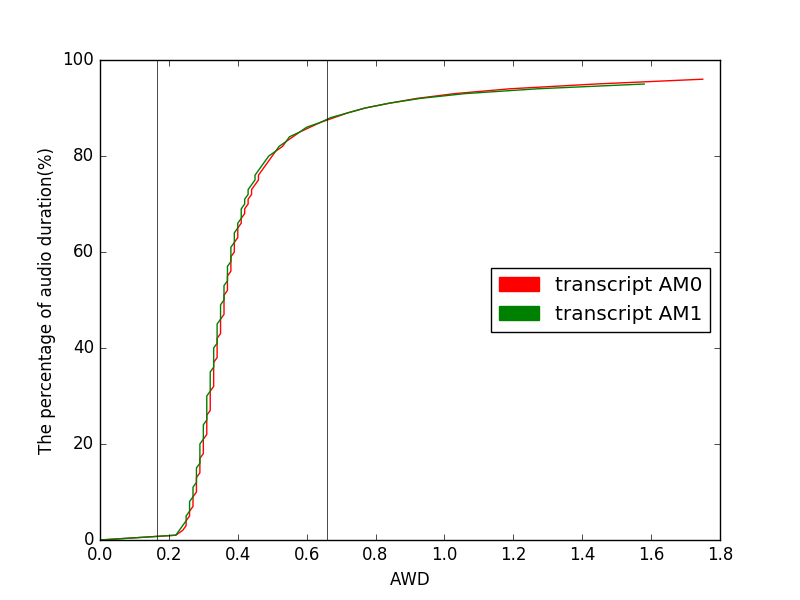
\includegraphics[scale=0.7]{awdLineChart}
\centering
\end{figure}

\begin{figure}
\caption{Phone match error rate}
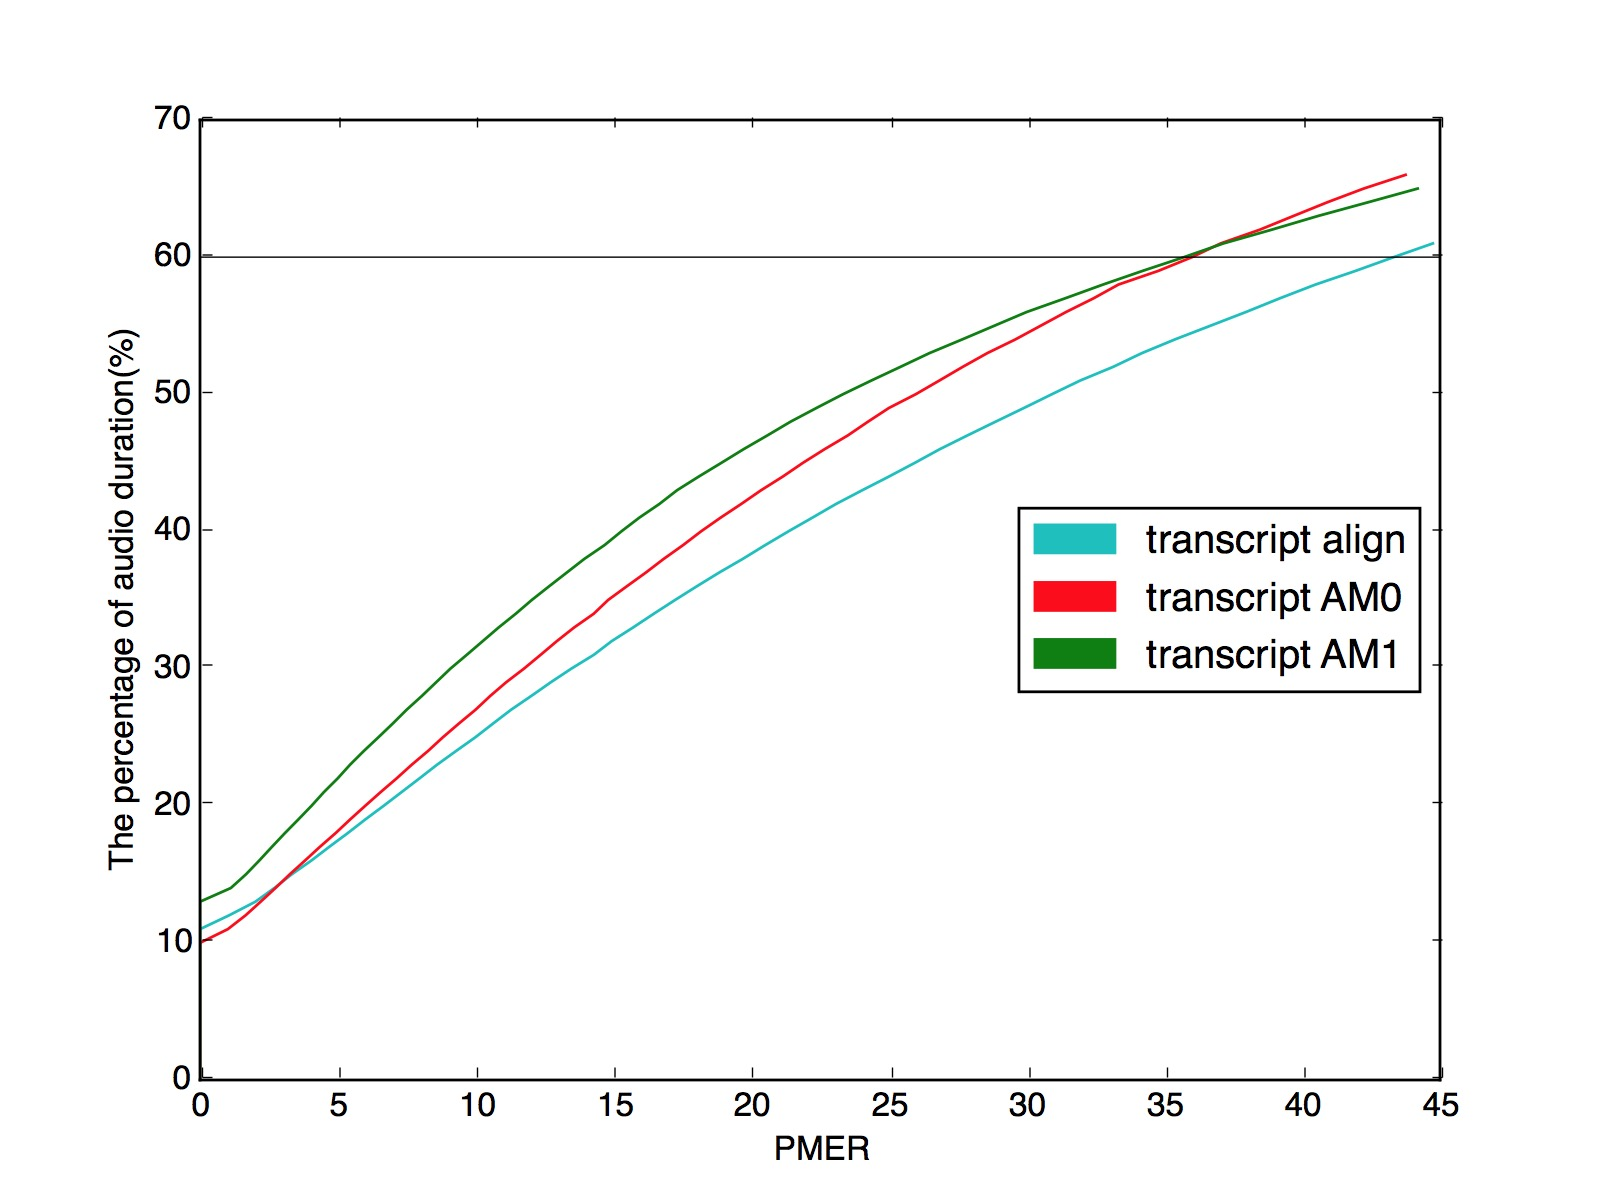
\includegraphics[scale=0.3]{pmerLineChart}
\centering
\end{figure}

\begin{figure}
\caption{Word match error rate}
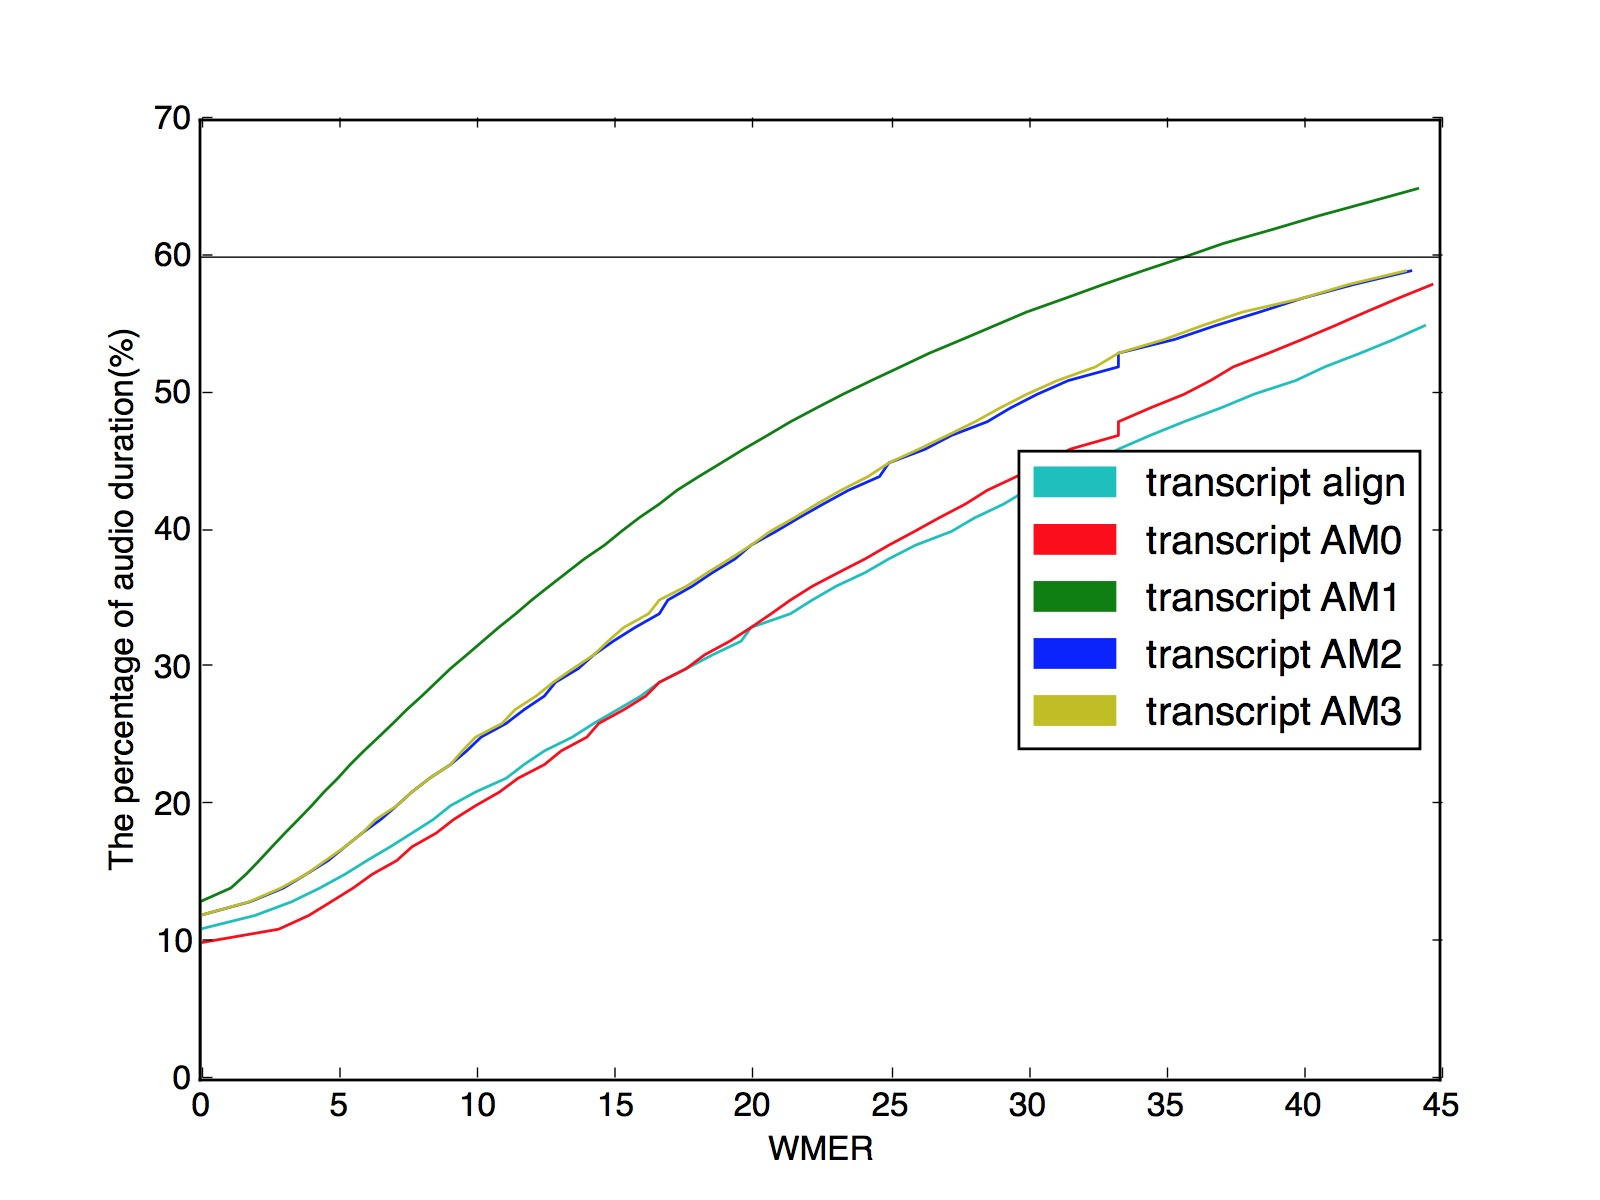
\includegraphics[scale=0.25]{wmerLineChart}
\centering
\end{figure}




%PER 32.2 | 9118 204786 | 75.0 10.0 15.0 7.2 32.2 82.7 | -1.058 | |
%WER 49.3 | 9118 64248 | 59.0 25.1 15.9 8.2 49.3 83.7 | -0.822 | |

%AM0_s1
%WMER
%[0, 0.05001182297101408, 0.1000055705823501, 0.15002999947778156, 0.20000377990423135, 0.250006911717846, 0.3000083202847346, 0.350008061797726, 0.4000080655439148, 0.45000218777410367, 0.5000070802963298, 0.5500076834326855, 0.6000113209817511, 0.6500022214898035, 0.7000031243212423, 0.7500004870045146, 0.8000498093227562, 0.8500152732106541]
%[0, 0.0, 0.0, 0.05, 0.08, 0.12, 0.15, 0.19, 0.23, 0.27, 0.32, 0.37, 0.43, 0.5, 0.58, 0.71, 0.98, 4.67]

%PMER
%[0, 0.05000255115439209, 0.10000343525488571, 0.15000458158857732, 0.20000319924500873, 0.2500218028172682, 0.3000072338900607, 0.3500012437345947, 0.4000032891535333, 0.45000364878763255, 0.5000033341077957, 0.5500060913025576, 0.6000314567451253, 0.6500026335705453, 0.700001251226977, 0.7500149847541436, 0.8000220313347739, 0.8500007005372576]
%[0, 0.0, 0.0, 0.02, 0.05, 0.07, 0.1, 0.13, 0.16, 0.2, 0.24, 0.28, 0.33, 0.39, 0.47, 0.59, 0.82, 4.43]

%Align
%WMER
%([0, 0.050002832118532126, 0.10000931677088468, 0.15000742869186362, 0.20000679558600154, 0.2500274408310134, 0.30000118379557716, 0.3500026485552931, 0.40000639849001596, 0.4500279240893308, 0.5000118004938804, 0.5500090133296115, 0.6000040159141051, 0.6500046752432919, 0.7000030681284111, 0.7500003184260248, 0.800006522114234], [0, 0.0, 0.0, 5.26, 9.09, 13.51, 17.65, 22.22, 27.27, 32.43, 38.24, 44.44, 52.17, 61.11, 72.73, 88.89, 108.33], 'b-'

%PMER
%[0, 0.05001950265750902, 0.10000225520549781, 0.15000134113549585, 0.20000690797165727, 0.25000294075800095, 0.30001437037921774, 0.35000064434442896, 0.40001250477732614, 0.45001977612927163, 0.5000107890229769, 0.5500005656744683, 0.60003347968693, 0.6500121301584764, 0.7000086499493287, 0.7500019667489803, 0.800000340903153], [0, 0.0, 0.0, 3.33, 6.67, 10.0, 13.48, 17.24, 21.35, 25.94, 30.91, 36.67, 43.32, 51.52, 61.82, 76.47, 100.0], 'r-'

 
\chapter{Sample Title}

Lorem ipsum dolor sit amet, consectetur adipiscing elit, sed do eiusmod tempor incididunt ut labore et dolore magna aliqua. Ut enim ad minim veniam, quis nostrud exercitation ullamco laboris nisi ut aliquip ex ea commodo consequat. Duis aute irure dolor in reprehenderit in voluptate velit esse cillum dolore eu fugiat nulla pariatur. Excepteur sint occaecat cupidatat non proident, sunt in culpa qui officia deserunt mollit anim id est laborum.

%now enable appendix numbering format and include any appendices
%\appendix
%\chapter{Sample Title}

Lorem ipsum dolor sit amet, consectetur adipiscing elit, sed do eiusmod tempor incididunt ut labore et dolore magna aliqua. Ut enim ad minim veniam, quis nostrud exercitation ullamco laboris nisi ut aliquip ex ea commodo consequat. Duis aute irure dolor in reprehenderit in voluptate velit esse cillum dolore eu fugiat nulla pariatur. Excepteur sint occaecat cupidatat non proident, sunt in culpa qui officia deserunt mollit anim id est laborum.
%\chapter{Sample Title}

Lorem ipsum dolor sit amet, consectetur adipiscing elit, sed do eiusmod tempor incididunt ut labore et dolore magna aliqua. Ut enim ad minim veniam, quis nostrud exercitation ullamco laboris nisi ut aliquip ex ea commodo consequat. Duis aute irure dolor in reprehenderit in voluptate velit esse cillum dolore eu fugiat nulla pariatur. Excepteur sint occaecat cupidatat non proident, sunt in culpa qui officia deserunt mollit anim id est laborum.

%next line adds the Bibliography to the contents page
\addcontentsline{toc}{chapter}{Bibliography}
%uncomment next line to change bibliography name to references
%\renewcommand{\bibname}{References}
\bibliography{refs}        %use a bibtex bibliography file refs.bib
\bibliographystyle{plain}  %use the plain bibliography style

\end{document}

